\documentclass[twoside]{article}
\usepackage[svgnames]{xcolor}
\usepackage{ctex}
\usepackage{amsmath}
\usepackage{graphicx}
\usepackage[top=1.25in,bottom=1.25in,outer=1in,inner=1.25in,a4paper]{geometry}
\usepackage{unicode-math}
\usepackage{tcolorbox}
\usepackage{fontspec}
\usepackage{tikz}
\usepackage{pgfplots}
\usepackage{mathtools}
\usepackage{pxrubrica}
\usepackage{fancyhdr}
\usepackage{ulem}
\usepackage{mleftright}
\usepackage{enumitem}
\usepackage{titlesec}
\usepackage{zhlipsum}
\usepackage{xfakebold}
\usepackage{microtype}
\usepackage{ifthen}
\usepackage{amsthm}
\usepackage{lettrine}
\usepackage{calc}
\usepackage{layout}
\usepackage{lastpage}
\usepackage{lipsum}
\usepackage{hyperref}
\usepackage{xint,xintcore,xinttools,xintexpr}
\usepackage{xfp}
\usepackage{numerica}
\usepackage{listings}
\usepackage{tabularray}
\usepackage{manfnt}
\usepackage{xltxtra}
\usepackage{simpleicons}
\usetikzlibrary{patterns}
\tcbuselibrary{skins} 
\tcbuselibrary{breakable}
\tcbuselibrary{theorems}
\tcbuselibrary{most}


\everymath{\displaystyle}
\makeatletter
\providecommand{\xlongequal}[2][]{\ext@arrow 0099{\arrowfill@===}{#1}{#2}}
\renewenvironment{proof}[2]{\begin{prof}{#1}{}\pushQED{\qed}\normalfont\topsep6\p@\@plus6\p@\relax\trivlist\item #2\@addpunct{.}}{\popQED\endtrivlist\@endpefalse\end{prof}}
\renewenvironment{cases}[1]{\begin{dcases}#1}{\end{dcases}}

\newenvironment{thoerem}[2]{\par\begin{flushright}\begin{theo}{#1}{}\trivlist\item #2}{\end{theo}\end{flushright}}

\renewenvironment{quote}[1]{\begin{flushright}\vskip-1.56em\begin{tcolorbox}[enforce breakable,colback=gray!20,colframe=gray!100,fonttitle=\bfseries,arc=0mm,leftrule=2pt,toprule=0mm,bottomrule=0mm,rightrule=0mm,before upper=\small,overlay first={\filldraw[line width=2pt,color=gray!100,rounded corners]([yshift=-1pt]frame.north west)--([yshift=-1pt,xshift=-30pt]frame.north west)--([yshift=-32mm,xshift=-30pt]frame.north west)--([yshift=-32mm,xshift=0mm]frame.north west)--([yshift=0mm,xshift=0mm]frame.north west);\draw[line width=2pt,color=gray!100] ([yshift=-32mm,xshift=-4pt]frame.north west)--([yshift=-32mm,xshift=0mm]frame.north west)--([yshift=0mm,xshift=0mm]frame.north west);\node[label=center:{\color{white}{\Huge{\textit{\textbf{Q}\,}}}\rule{2pt}{80pt}}]at([yshift=-15.1mm,xshift=-5mm]frame.north west){};},width=0.95\linewidth,left=15pt,enhanced jigsaw,use color stack,colupper=darkgray]\itshape #1}{\end{tcolorbox}\end{flushright}}
\@namedef{nameenglishtest@A}{\raise0.42ex\hbox{\bfseries\ebgaramondinitialswithdout{A}}}
\@namedef{nameenglishtest@Q}{\raise0.42ex\hbox{\bfseries\ebgaramondinitialswithdout{Q}}}
\@namedef{nameenglishtest@D}{\raise0.42ex\hbox{\bfseries\ebgaramondinitialswithdout{D}}}
\@namedef{nameenglishtest@T}{\raise0.42ex\hbox{\bfseries\ebgaramondinitialswithdout{T}}}
\@namedef{nameenglishtest@F}{\raise0.42ex\hbox{\bfseries\ebgaramondinitialswithdout{F}}}
\@namedef{nameenglishtest@G}{\raise0.42ex\hbox{\bfseries\ebgaramondinitialswithdout{G}}}
\@namedef{nameenglishtest@L}{\raise0.42ex\hbox{\bfseries\ebgaramondinitialswithdout{L}}}
\@namedef{nameenglishtest@N}{\raise0.42ex\hbox{\bfseries\ebgaramondinitialswithdout{N}}}
\@namedef{nameenglishtest@O}{\raise0.42ex\hbox{\bfseries\ebgaramondinitialswithdout{O}}}
\newcommand{\nameenglishtest}[1]{\expandafter\ifx\csname nameenglishtest@#1\endcsname\relax\bfseries\ebgaramondinitialswithdout#1\kern-0.2ex\else\csname nameenglishtest@#1\endcsname\fi}
\makeatother

\pagestyle{fancy}

\newfontfamily{\ebgaramondinitialswithdout}{EBGaramond-Initials.otf}
\setmainfont{EB Garamond}[RawFeature={+calt,+liga,+hlig,+clig,+dlig,+tnum,+lnum}]
\setmathfont{Garamond-Math.otf}[StylisticSet={7, 9}]
\setmathfont{Garamond-Math.otf}[StylisticSet={7, 9, 8}, version=a]
\setmathfont[range="0211C]{Latin Modern Math}

\setsansfont{Ysabeau Office}
\setCJKmainfont{FZFW ZhuZi A Old Mincho R}[ItalicFont = FZKaiS-Extended]
\setCJKsansfont{HarmonyOS Sans SC}
\setCJKmonofont{HarmonyOS Sans SC Light}
\setmonofont{Iosevka}
\newCJKfontfamily{\tagJAP}{FOT-TsukuOldMin Pro}
\newfontface\emojifontsettings{Seguiemj.ttf}

\newcommand{\eater}[1]{}

\newlength{\fortest}
\settowidth{\fortest}{\hspace{2.25cm}}
\renewcommand{\relbar}{\symbol{"E010}\mkern-.2mu\symbol{"E010}\mkern1.8mu}
\renewcommand{\Relbar}{\symbol{"E011}\mkern-.2mu\symbol{"E011}\mkern1.8mu}
\newcommand{\ebgaramondinitials}[2]{\lettrine{\!\nameenglishtest{#1}\!}{\,\kern0.5em#2}}
\newcommand{\emoji}[1]{{\emojifontsettings#1}}
\DeclareMathOperator{\besselj}{\,J}  
\DeclareMathOperator{\bessely}{Y}
\DeclareMathOperator{\Ai}{Ai}  
\DeclareMathOperator{\Bi}{Bi}
\DeclareMathOperator{\laplace}{\symcal{L}}
\DeclareMathOperator*{\diam}{diam}
\DeclareMathOperator{\card}{card}

\newcommand{\sectionabstract}[1]
{
	\ifthenelse{\isodd{\value{page}}}
	{
		\ifthenelse{\value{sectionindex}<10}
		{
			\settowidth{\abswidth}{\parbox{23em}{\small\itshape #1}}
			\settoheight{\absheight}{\parbox{23em}{\small\itshape #1}}\ifthenelse{\lengthtest{\absheight > 2.25cm}}{\vspace{\absheight - \fortest + 1cm}}{}
			\begin{tikzpicture}[overlay, remember picture]
			\node [yshift=-4.25cm - \absheight, xshift = 5.2cm + 0.5\abswidth] at (current page.north west){\parbox{23em}{\small\itshape #1}};
			\end{tikzpicture}
		}
		{
			\settowidth{\abswidth}{\parbox{18em}{\small\itshape #1}}
			\settoheight{\absheight}{\parbox{18em}{\small\itshape #1}}\ifthenelse{\lengthtest{\absheight > 2.25cm}}{\vspace{\absheight - \fortest + 1cm}}{}
			\begin{tikzpicture}[overlay, remember picture]
			\node [yshift=-4.25cm - \absheight, xshift = 5.2cm + 0.5\abswidth] at (current page.north west){\parbox{18em}{\small\itshape #1}};
			\end{tikzpicture}
		}
	}
	{
		\ifthenelse{\value{sectionindex} < 10}
		{
			\settowidth{\abswidth}{\parbox{23em}{\small\itshape #1}}
			\settoheight{\absheight}{\parbox{23em}{\small\itshape #1}}\ifthenelse{\lengthtest{\absheight > 2.25cm}}{\vspace{\absheight - \fortest + 1cm}}{}
			\begin{tikzpicture}[overlay, remember picture]
			\node [yshift=-4.25cm - \absheight, xshift = \paperwidth - 5.2cm - 0.5\abswidth] at (current page.north west){\parbox{23em}{\small\itshape #1}};
			\end{tikzpicture}
		}
		{
			\settowidth{\abswidth}{\parbox{18em}{\small\itshape #1}}
			\settoheight{\absheight}{\parbox{18em}{\small\itshape #1}}\ifthenelse{\lengthtest{\absheight > 2.25cm}}{\vspace{\absheight - \fortest + 1cm}}{}
			\begin{tikzpicture}[overlay, remember picture]
			\node [yshift=-4.25cm - \absheight, xshift =\paperwidth - 5.2cm - 0.5 * \abswidth] at (current page.north west){\parbox{18em}{\small\itshape #1}};
			\end{tikzpicture}
		}
	}
}
\renewcommand{\contentsname}{\textit{\Huge CONTENT}}

\let\left\mleft
\let\right\mright

\fancypagestyle{forsection}
{
\fancyhf{}
\renewcommand{\headrulewidth}{0pt}
\fancyfoot[RO]{\vskip-8em\rotatebox[origin=rb]{-90}{{\LARGE\char"2619}\enspace{\bfseries\Roman{page}}\enspace{\LARGE\char"2767}}\kern-3em}
\fancyfoot[LE]{\vskip-8em\hspace{-3em}\rotatebox[origin=lb]{90}{{\LARGE\char"2619}\enspace{\bfseries\Roman{page}}\enspace{\LARGE\char"2767}}}
\fancyhead[C]{}
}

\fancyfoot[RO]{\vskip-8em\rotatebox[origin=c]{-90}{{\LARGE\char"2619}\enspace{\bfseries\Roman{page}}\enspace{\LARGE\char"2767}}\kern-2.5em}
\fancyfoot[LE]{\vskip-8em\hspace{-2.5em}\rotatebox[origin=c]{90}{{\LARGE\char"2619}\enspace{\bfseries\Roman{page}}\enspace{\LARGE\char"2767}}}
\fancyhead[C]{}
\fancyfoot[C]{}
\fancyfoot[CO]
{
	\begin{tikzpicture}[remember picture,overlay]
		\node[yshift=-2.25cm] at (current page.north west)
		{
			\begin{tikzpicture}[remember picture, overlay]
			% \draw[draw=gray!150,line width = 2pt] (\paperwidth-0.625cm,2.5cm) -- (\paperwidth - 0.625cm, -\value{sectionindex} * 1cm + 1cm);
			\draw[fill = gray!150,draw=none] (\paperwidth-1.25cm,-\value{sectionindex} * 1cm) rectangle (\paperwidth, -\value{sectionindex} * 1cm + 1cm) node[xshift = -0.625cm, yshift = -0.5cm] {\color{white}\Large\arabic{sectionindex}};
			\end{tikzpicture}
		};
	\end{tikzpicture}
}
\fancyfoot[CE]
{
	\begin{tikzpicture}[remember picture,overlay]
		\node[yshift=-2.25cm] at (current page.north west){
			\begin{tikzpicture}[remember picture, overlay]
				% \draw[draw=gray!150,line width = 2pt](0.625cm, -\paperheight) -- (0.625cm, -\value{sectionindex} * 1cm + 1cm);
			\draw[fill = gray!150,draw=none] (0cm,-\value{sectionindex} * 1cm) rectangle (1.25cm, -\value{sectionindex} * 1cm + 1cm) node[xshift = -0.625cm, yshift = -0.5cm] {\color{white}\Large\arabic{sectionindex}};
		\end{tikzpicture}
		};
	\end{tikzpicture}
}

\newcounter{para}
\setcounter{para}{1}
\newlength{\paralength}
\newlength{\raw}
\newlength{\slashlength}
\newlength{\abswidth}
\newlength{\absheight}

\def\uppartial{\symup\partial}
\titleformat{\subsection}[hang]{}{\ifthenelse{\value{subsection}>9}{\normalsize\filright\raisebox{-1.3ex}{\huge\char"B6}\kern-2.3ex\raisebox{0.2ex}{\rotatebox[origin=c]{-90}{\color{white}\footnotesize\arabic{subsection}}}}{\normalsize\filright\raisebox{-1.3ex}{\huge\char"B6}\kern-2.3ex{\color{white}\normalsize\arabic{subsection}}}\enspace}{0.5em}{\normalsize\bfseries}
\titleformat{\paragraph}[runin]{}{}{}{\settowidth{\paralength}{\arabic{para}}\hspace{-\paralength}\bfseries\arabic{para}\hspace{-\paralength}\kern1.5em\char"261E\kern1ex\stepcounter{para}\,}[]

\newcounter{sectionindex}

\titleformat{\section}[display]{}
{
	\newpage
	\ifthenelse{\isodd{\value{page}}}
	{
		\ifthenelse{\value{section} < 10}
		{
			\begin{tikzpicture}[remember picture,overlay]
				\node[yshift=-3 .25cm] at (current page.north west)
				{
					\begin{tikzpicture}[remember picture, overlay]
						\draw[fill = gray!80,draw=none] (5cm , 0cm) rectangle (\paperwidth , 1cm);
						\draw[fill = gray!80,draw=none] (5cm , -0.5cm) rectangle (\paperwidth , -0.3cm);
					\end{tikzpicture}
				};
				\node[yshift=-7.25cm] at (current page.north west)
				{
					\begin{tikzpicture}[remember picture, overlay]
						\draw[fill = gray!20,draw=none] (\paperwidth-6.25cm , 0cm) rectangle (\paperwidth-3.25cm, 7.3cm);
					\end{tikzpicture}
				};
			\end{tikzpicture}
			\setcounter{sectionindex}{\thesection}
			\thispagestyle{forsection}\filleft\fontsize{100pt}{0pt}\textbf{\textit{\arabic{section}}}\hspace{3em}
		}
		{
			\begin{tikzpicture}[remember picture,overlay]
				\node[yshift=-3.25cm] at (current page.north west)
				{
					\begin{tikzpicture}[remember picture, overlay]
						\draw[fill = gray!80,draw=none] (5cm , 0cm) rectangle (\paperwidth , 1cm);
						\draw[fill = gray!80,draw=none] (5cm , -0.5cm) rectangle (\paperwidth , -0.3cm);
					\end{tikzpicture}
				};
				\node[yshift=-7.25cm] at (current page.north west)
				{
					\begin{tikzpicture}[remember picture, overlay]
						\draw[fill = gray!20,draw=none] (\paperwidth-8.25cm , 0cm) rectangle (\paperwidth-3.25cm, 7.3cm);
					\end{tikzpicture}
				};
			\end{tikzpicture}
			\setcounter{sectionindex}{\thesection}
			\thispagestyle{forsection}\filleft\fontsize{100pt}{0pt}\textbf{\textit{\arabic{section}}}\hspace{3em}
		}
	}
	{
		\ifthenelse{\value{section} < 10}
		{
			\begin{tikzpicture}[remember picture,overlay]
				\node[yshift=-3 .25cm] at (current page.north west)
				{
					\begin{tikzpicture}[remember picture, overlay]
						\draw[fill = gray!80,draw=none] (0cm , 0cm) rectangle (\paperwidth -5cm, 1cm);
						\draw[fill = gray!80,draw=none] (0cm , -0.5cm) rectangle (\paperwidth -5cm, -0.3cm);
					\end{tikzpicture}
				};
				\node[yshift=-7.25cm] at (current page.north west){
					\begin{tikzpicture}[remember picture, overlay]
						\draw[fill = gray!20,draw=none] (3.25cm , 0cm) rectangle (6.25cm, 7.3cm);
					\end{tikzpicture}
				};
			\end{tikzpicture}
			\setcounter{sectionindex}{\thesection}
			\thispagestyle{forsection}\filright\fontsize{100pt}{0pt}\hspace{3em}\textbf{\textit{\arabic{section}}}
		}
		{
			\begin{tikzpicture}[remember picture,overlay]
				\node[yshift=-3 .25cm] at (current page.north west)
				{
					\begin{tikzpicture}[remember picture, overlay]
						\draw[fill = gray!80,draw=none] (0cm , 0cm) rectangle (\paperwidth -5cm, 1cm);
						\draw[fill = gray!80,draw=none] (0cm , -0.5cm) rectangle (\paperwidth -5cm, -0.3cm);
					\end{tikzpicture}
				};
				\node[yshift=-7.25cm] at (current page.north west)
				{
					\begin{tikzpicture}[remember picture, overlay]
						\draw[fill = gray!20,draw=none] (3.25cm , 0cm) rectangle (8.25cm, 7.3cm);
					\end{tikzpicture}
				};
			\end{tikzpicture}
			\setcounter{sectionindex}{\thesection}
			\thispagestyle{forsection}\filright\fontsize{100pt}{0pt}\hspace{3em}\textbf{\textit{\arabic{section}}}
		}
	}
}{4em}{\ifthenelse{\isodd{\value{page}}}{\vskip-3em\phantom{d}\kern-3em\mbox\bgroup\Large\bfseries\rightline}{\vskip-3em\phantom{d}\kern2em\mbox\bgroup\Large\bfseries}}[\egroup\vspace{3em}]


\defaultfontfeatures{RawFeature={+swsh}}

% \catcode`\,=13
% \def,{, }
% \catcode`\、=13
% \def、{\mbox{\char"3001\kern-0.25em}}
\catcode`\。=13
\def。{.}
% \catcode`\:=13
% \def:{: }
% \catcode`\;=13
% \def;{; }
% \catcode`\!=13
% \def!{\,!\,}
% \catcode`\?=13
% \def?{ ? }
\catcode`\(=13
\def({\raisebox{0.28ex}{\,(}}
\catcode`\)=13
\def){\raisebox{0.28ex}{)\,}}
% \catcode`\“=13
% \def“{``}
% \catcode`\”=13
% \def”{''}
% \catcode`\、=13
% \def、{\mbox{\char"3001\kern-0.35em}}
% \catcode`\「=13
% \def「{\mbox{\kern-0.35em\char"300C}}
% \catcode`\」=13
% \def」{\mbox{\char"300D\kern-0.35em}}

\newlength{\hollowlen}
\def\texthollow#1#2{\settowidth{\hollowlen}{#2}\setBold[#1] #2\unsetBold\kern-\hollowlen{\color{white}#2}}

\newtcbtheorem[number within=section]{prof}{PROOF}{colback=gray!20,colframe=gray!150,fonttitle=\bfseries,arc=0mm,leftrule=0mm,toprule=0mm,bottomrule=1mm,rightrule=0mm,breakable}{prof}

\newtcbtheorem[number within=section]{theo}{THEOREM}{attach boxed title to top left={yshift=-9.18pt,xshift=0pt},colback=gray!20,colframe=gray!100,fonttitle=\bfseries,breakable,boxed title style={sharp corners},enhanced,arc=0mm,boxrule=0pt,boxed title style={size=minimal,toprule=0pt,top=4pt,bottom=4pt,left=4pt,right=4pt,overlay={\filldraw[gray!50!black,line width=0pt,fill=gray!100]([yshift=-1pt, xshift=-1pt]frame.north east)--([yshift=-1pt]frame.north east)--([xshift=8pt,yshift=-1pt]frame.east)--([xshift=0pt]frame.south east)--([xshift=-2pt]frame.south east);\draw[gray!50!black,line width=2pt]([yshift=-1pt]frame.north west)--([yshift=-1pt]frame.north east)--([xshift=8.5pt,yshift=-0.5pt]frame.east);}},coltitle=white,leftrule=2pt,width=0.95\linewidth,boxsep=0pt,top=17pt}{theo}


\begin{document}
\let\symcal\relax
\setlength{\lineskip}{5pt}
\setlength{\lineskiplimit}{2.5pt}
\DeclareRobustCommand{\mathhollow}[1]{\mathpalette\mathhollowker{#1}}
\newcommand{\mathhollowker}[2]{\settowidth{\hollowlen}{\(#1#2\)}\setBold[0.5] #2\unsetBold\kern-\hollowlen{\color{white}#2}}

\DeclareRobustCommand{\symcal}[1]{{\mathpalette\justsetupthemathcalfont{#1}}}
\newcommand{\justsetupthemathcalfont}[2]{\mbox{\mathversion{a}\(#1\symscr{#2}\)}}

\DeclareRobustCommand{\nlongrightrightarrows}{\mathpalette\nllraw\relax}
\DeclareRobustCommand{\longrightrightarrows}{\mathpalette\llraw\relax}
\DeclareRobustCommand{\nlongrightarrow}{\mathpalette\nlraw\relax}
\newcommand{\llraw}[1]{\settowidth{\raw}{\(#1\longrightarrow\)}\mathrel{\raisebox{-0.11\raw}{\(#1\longrightarrow\)} \hspace{-\raw}\raisebox{0.11\raw}{\(#1\longrightarrow\)}}}
\newcommand{\nlraw}[1]{\settowidth{\raw}{\(#1\longrightarrow\)}\settowidth{\slashlength}{\(#1/\)}#1\longrightarrow\hspace{-0.7\raw}/\hspace{0.7\raw-\slashlength}}
\newcommand{\nllraw}[1]{\settowidth{\raw}{\(#1\longrightarrow\)}\settowidth{\slashlength}{\(#1/\)}\mathrel{\raisebox{-0.11\raw}{\(#1\longrightarrow\)} \hspace{-\raw}\raisebox{0.11\raw}{\(#1\longrightarro\)}\hspace{-0.7\raw}/\hspace{0.7\raw-\slashlength}}}
\everymath{\displaystyle}

\gdef\pi{\symup π}
\gdef\partial{\symup ∂}
\gdef\gamma{\symup γ}

\setcounter{page}{1}

\pagestyle{empty}
\begin{tikzpicture}[overlay, remember picture]
	\filldraw[fill = Gold, line width = 0pt, color = Gold] (current page.south west) rectangle ([yshift = -0.4\paperwidth]current page.north east);
	\node at ([xshift = 0.5\paperwidth, yshift = -0.8\paperwidth]current page.north west) {
		\begin{minipage}{40em}
			\fontsize{30pt}{30pt}\selectfont
			\textbf{\textsf{Innocent FIVE}}\\\vskip10pt
			\fontsize{70pt}{50pt}\selectfont
			\textbf{\kern-5pt\textsf{BABY}}\\
			\fontsize{50pt}{50pt}\selectfont
			\textbf{\kern-8pt\textsf{Complex Function}}\\
			\fontsize{30pt}{20pt}\selectfont
			\textbf{\textsf{Editions}}\\
			\fontsize{30pt}{40pt}\selectfont
			\textit{卑鄙的复变函数}
		\end{minipage}
	};
	\node at ([xshift = 15em, yshift = 10em]current page.south west) {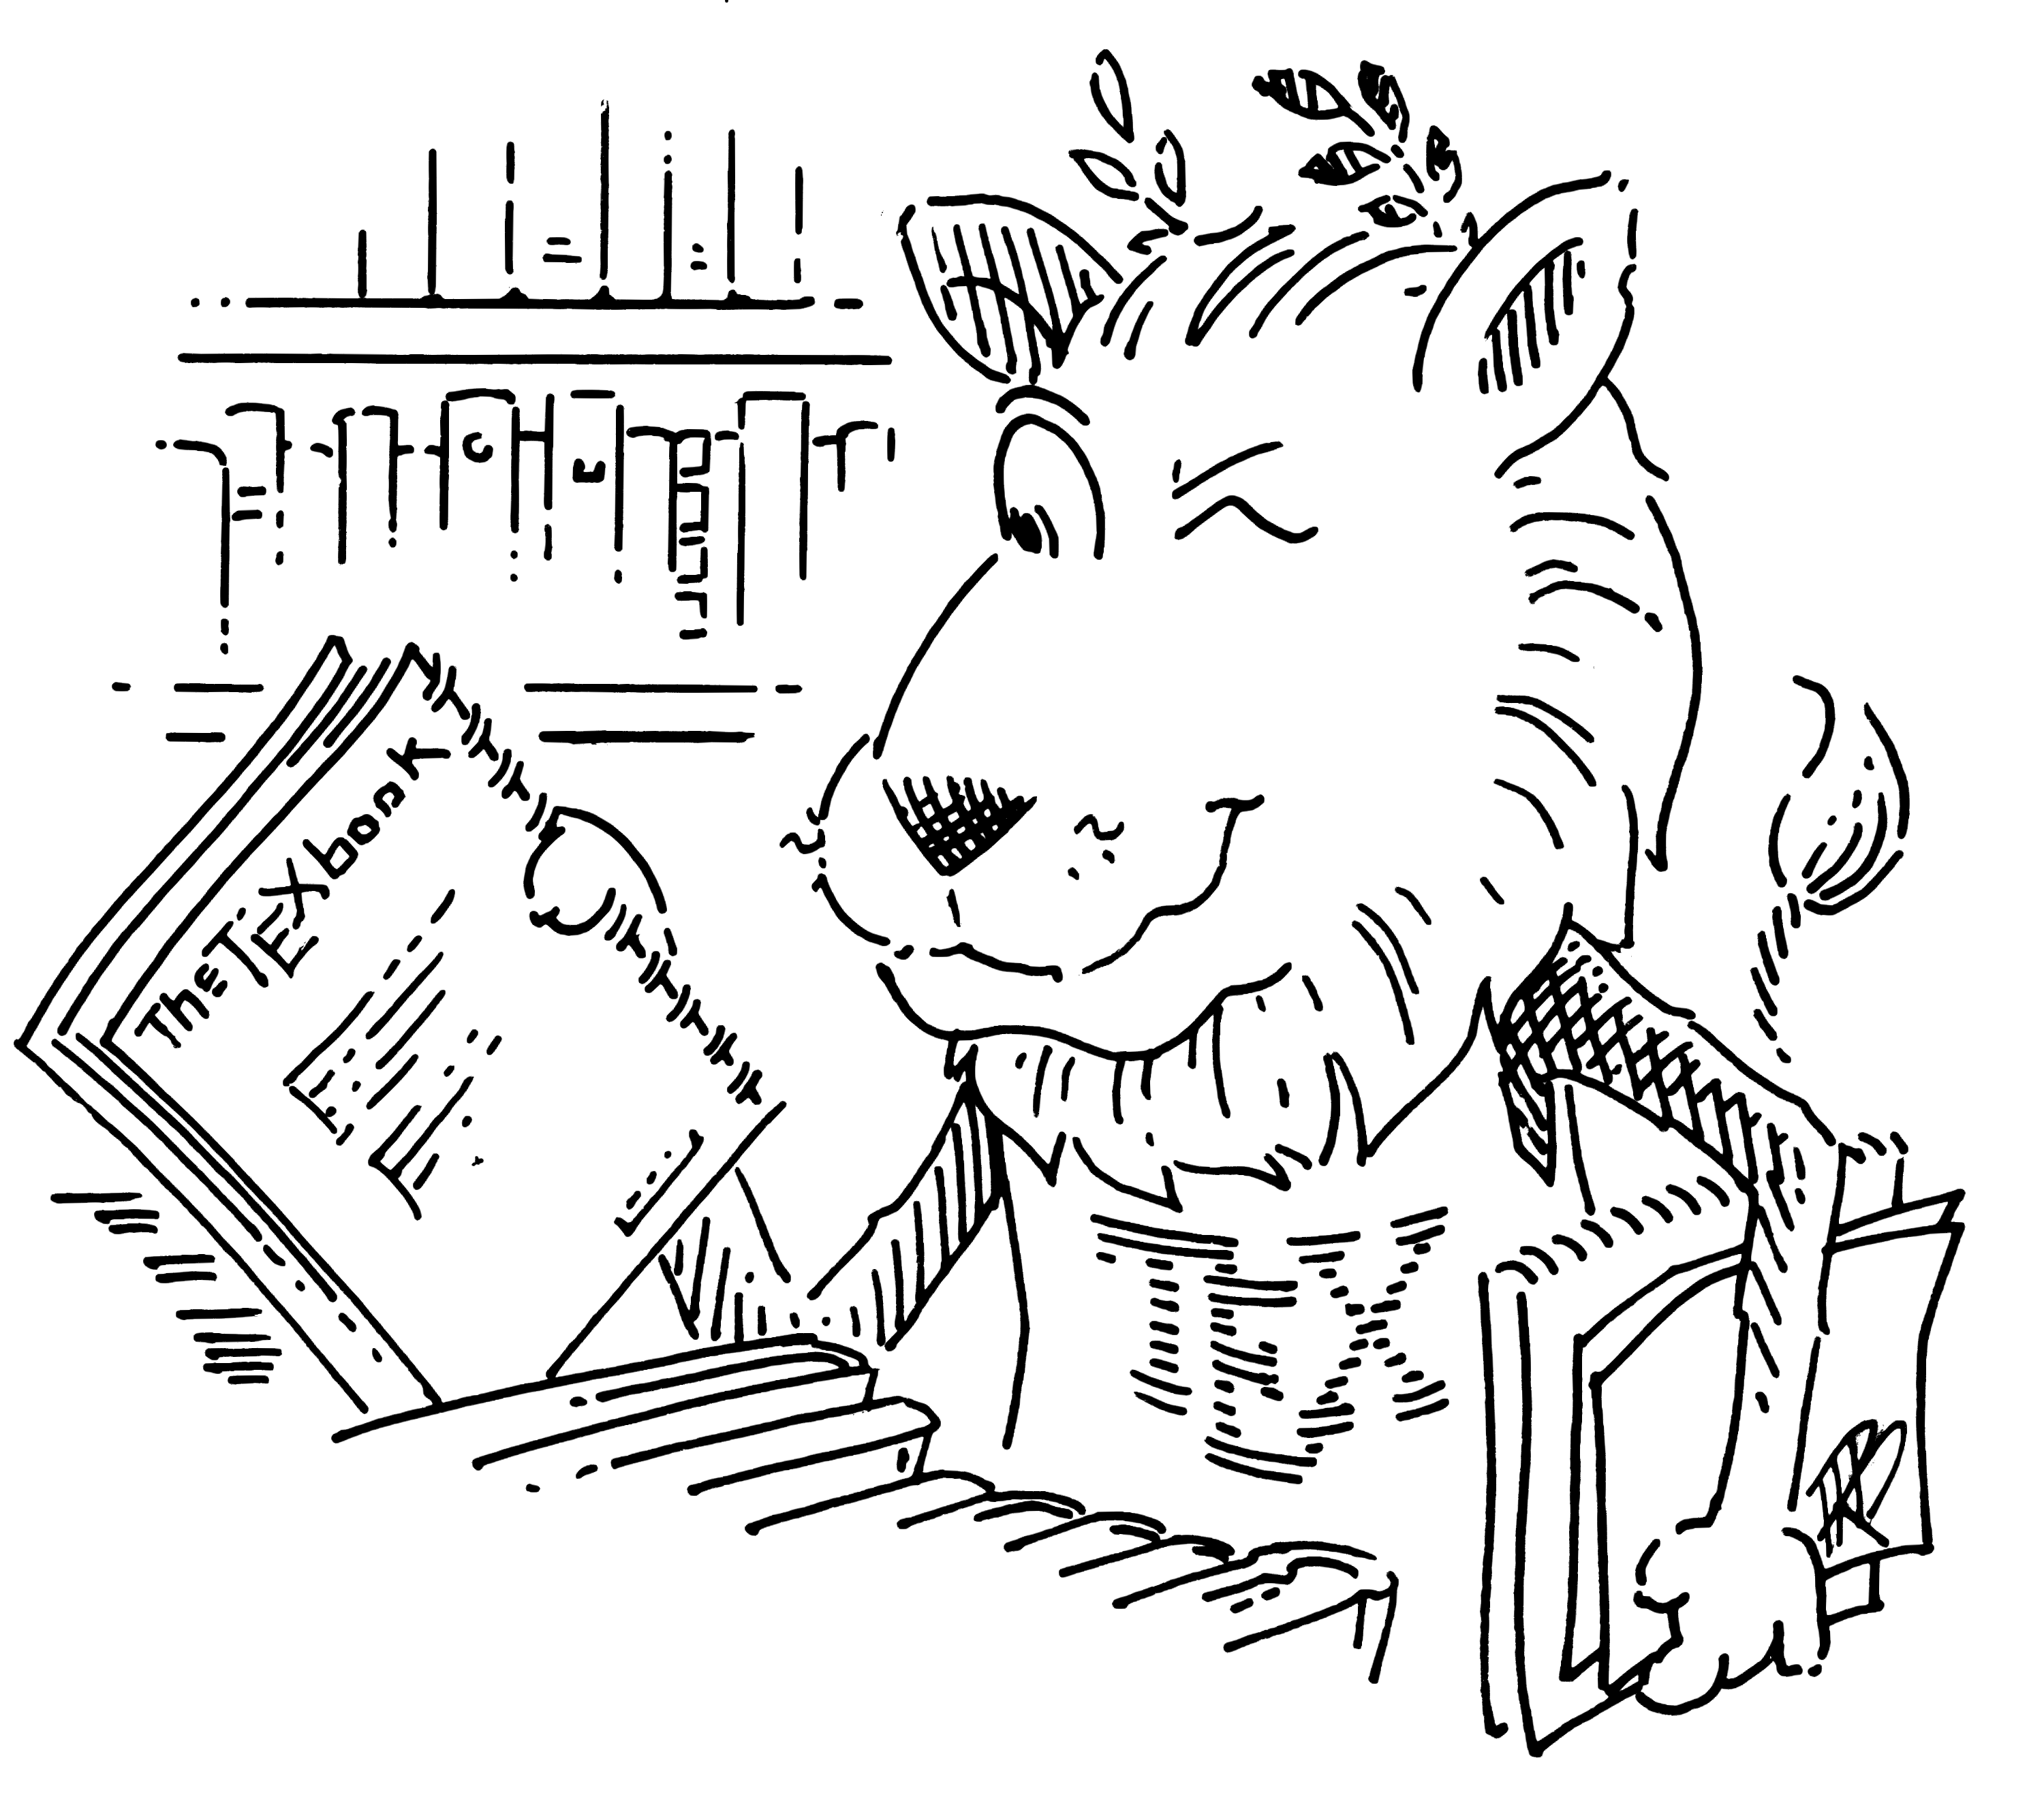
\includegraphics[width = 12em]{LION.png}};
	\node at ([xshift = 25em, yshift = 10em]current page.south west) {\Huge\XeLaTeX};
	\node at ([xshift = -0.5\paperwidth, yshift = -0.2\paperwidth]current page.north east) {\color{Gold}\fontsize{150pt}{50pt}\simpleicon{mcdonalds}};
\end{tikzpicture}



\newpage

\tableofcontents
\newpage
\pagestyle{fancy}
% \newpage
% \pagestyle{fancy}
\section*{序}

\lettrine{\textbf{这}}{\kern0.55em是工科复变笔记}并没有什么实质性的内容,因此会用极低的严谨性来介绍东西。另外的是,可能写错。

\begin{center}
	{\Huge \textbf{写错就写错吧!雨我无瓜。}}
\end{center}

项目地址会放在 \hyperref[https://github.com/InnocentFIVE/BABY-Complex-function]{https://github.com/InnocentFIVE/BABY-Complex-function}。

% % \begin{tblr}{width = \textwidth, colspec = {X[8]X[2]}}
% % \textbf{MIT License}
% % &
% % \\
% % Permission is hereby granted, free of charge, to any person obtaining a copy
% % of this software and associated documentation files (the ``Software"), to deal
% % in the Software without restriction, including without limitation the rights
% % to use, copy, modify, merge, publish, distribute, sublicense, and/or sell
% % copies of the Software, and to permit persons to whom the Software is
% % furnished to do so, subject to the following conditions: & 在这里允许所有人对这玩意干所有事(请别想歪),包括你能想到的各种奇妙事情,但必须:
% % \\

% % The above copyright notice and this permission notice shall be included in all
% % copies or substantial portions of the Software. & 保留这个许可。
% % \\

% % THE SOFTWARE IS PROVIDED ``AS IS", WITHOUT WARRANTY OF ANY KIND, EXPRESS OR
% % IMPLIED, INCLUDING BUT NOT LIMITED TO THE WARRANTIES OF MERCHANTABILITY,
% % FITNESS FOR A PARTICULAR PURPOSE AND NONINFRINGEMENT. IN NO EVENT SHALL THE
% % AUTHORS OR COPYRIGHT HOLDERS BE LIABLE FOR ANY CLAIM, DAMAGES OR OTHER
% % LIABILITY, WHETHER IN AN ACTION OF CONTRACT, TORT OR OTHERWISE, ARISING FROM,
% % OUT OF OR IN CONNECTION WITH THE SOFTWARE OR THE USE OR OTHER DEALINGS IN THE
% % SOFTWARE. & 这货出来就这样莉,没有任何保证,出了事别找我,雨我无瓜。
% % \end{tblr}
% \newpage
% \setlist{leftmargin = 4em}

\setcounter{page}{1}
\section{复数的形状}
\def\er{{\footnotesize 儿}}
\subsection{复数\er}
\lettrine{\textbf{复}\!}{\kern0.55em数}一般的形状长得像 \(x+ y\symrm{i} \),其中 \(x_1,y_1,x_2,y_2,m\in\symbb{R} \)。我们可以将其认为是一对\textbf{有序实数对} \((x,y)\) 满足:
\[
	\begin{cases}
		(x_1,y_1) + (x_2,y_2)= (x_1+x_2, y_1+y_2) ,                \\
		(x_1,y_1) \cdot (x_2,y_2 ) = (x_1x_2-y_1y_2,x_1y_2 + y_1x_2), \\
		m(x_1,y_1) = (mx_1,my_1).
	\end{cases}
\]
复数中存在加法单位元 \((0,0)\) ,乘法单位元 \((1,0)\),加法逆元 \((-x,-y) \),乘法逆元 \(\left( \frac{x}{x^2 +y^2 }, - \frac{y}{x^2 +y^2 } \right) \)。也满足一般的加法交换/结合律,乘法交换/结合/分配律。故这样的有序实数对的集合构成了一个域,称为\textbf{复数域}。记作 \(\symbb{C} \)。

复数没有良好的序关系,不能比较大小。

若一个复数表示为 \((a,b),\,a,b\in\symbb{R} \),我们定义:
\[
	\begin{cases}
		\Re((a,b)) \coloneqq  a , \\
		\Im((a,b)) \coloneqq  b.
	\end{cases}
\]
称为复数的\textbf{实部}和\textbf{虚部},显然实部和虚部都是\textbf{实数}。

为了方便书写,我们不妨定义:
\[
	\symrm{i} \coloneqq (0,1),\,\forall x\in\symbb{R} ,x=(x,0)
	.\]
考虑到复数域是对 \(\symbb{R} \) 的线性空间,我们可以写:
\[
	(a,b) = a+b\symrm{i}
	.\]
后者就是我们常见的写法,注意到这和Descartes二维坐标系有点像,我们也可以在坐标系上讨论复数:显然复数域有基 \((1,0) = 1\) 和 \((0,1) =\symrm{i} \)。他们张成一个平面:

\begin{center}
	\begin{tikzpicture}
		\tikzset{> = latex}
		\draw [->] (-5,0)--(5,0);
		\draw [->] (0,-3)--(0,3);
		\node [label = west:{\(\symrm{i}\)}](I) at (0,1){};
		\node [label = north:{\(1\)}](1) at (1,0){};
		\draw [->, thick] (0,0) -- (I.center);
		\draw [->, thick] (0,0) -- (1.center);
		\node [label = north east:{\(3+4\symrm{i} \)}] (P) at (4,3){};
		\draw [->] (0,0) -- (P.center);
	\end{tikzpicture}
\end{center}

称为\textbf{复平面}。

考虑 \(0 \cdot\symrm{i} =0_{\symbb{C} }\),这样一来我们默认不写 \(0 \cdot\symrm{i}\),即 \((3,0)\) 写成 \(3\) 而不是 \(3+0\symrm{i} \),且由于之前我们让 \((a,0)\) 记为 \(a\),因此可以尝试考虑在 \(\Im(z)=0\) 的复数 \(z\) 上定义实数的运算,包括绝对值等等,显然与复数定义相容。因此我们可以认为复数是实数的扩充,从而不再区分运算的所属关系,统一为复数运算。

但 \(\Im(z)\neq 0\) 时,复数与实数很不一样,此时需要定义一些运算:

\begin{itemize}
	\item 定义复数(由于复数是向量)的范(被称为复数的\textbf{模})与距离
	      \[
		      \begin{aligned}
			      d\left( \left( x_1,y_1 \right) ,\left( x_2,y_2 \right)  \right) & = \sqrt{\left( x_1-x_2 \right)^2+\left( y_1-y_2 \right) ^2 }, \\
			      \left| \left( x,y \right)  \right|                              & = \sqrt{x^2 +y^2 }.
		      \end{aligned}
	      \]
	\item 定义复数的\textbf{共轭}:
	      \[
		      \mathop{\rm Conj} (x,y) \coloneqq  (x,-y)
		      .\]
	      对一个复数 \(z\) 做共轭记为 \(z^*\)。
\end{itemize}
注意到和Descartes二维坐标系的范与距离一致,因此复数域变成了一个赋范空间。

我们暂且不讨论极限方面的内容,接下来是复数的极坐标表示,由于复平面与Descartes二维坐标系同构,我们同样可以采取极坐标来看待复数,首先定义辐角:
\[
	\arg z = \begin{cases}
		\theta, \mbox{\it 满足} \tan \theta= \frac{\Im(z)}{\Re(z)}  , & \Re(z) \neq 0             \\
		\frac{\pi}{2} + 2k \pi ,                                      & \Re(z)=0\land\Im(z)>0,    \\
		-\frac{\pi}{2} + 2k \pi ,                                     & \Re(z) = 0\land \Im(z)<0.
	\end{cases}\qquad k\in\symbb{Z}
\]
可以看到 \(0\) 的辐角我们是没有定义的。接下来我们同样会看到,由于辐角具有多值性,这会让讨论某些东西时非常麻烦。

因此我们暂且可以将复数用极坐标表示:
\[
	z =\left( \left| z \right|,\arg z \right)_{\rm P}  = \left\vert z \right\vert \left( \cos \arg z+\symrm{i} \sin \arg z \right) \sim r(\cos \theta+\symrm{i}  \sin \theta)
	.\]
注意到复数的乘法:
\[
	\begin{aligned}
		z_1\cdot z_2 & =  r_1 \left( \cos \theta_1+\symrm{i} \sin \theta_1 \right) r_2 \left( \cos \theta_2+\symrm{i} \sin \theta_2 \right)                                                                                                                                                 \\
		             & \xlongequal[\mbox{\tiny\it 交换/结合/分配性质}  ]{\mbox{\tiny\it 由于复数的}  }{} r_1 r_2 \left[ \left( \cos \theta_1 \cos \theta_2- \sin \theta_1 \sin \theta_2 \right)+\symrm{i} \left( \sin \theta_1 \cos \theta_2 +\sin \theta_2 \cos \theta_1 \right)   \right] \\
		             & = r_1r_2\left( \cos (\theta_1+\theta_2)+\symrm{i} \sin \left( \theta_1+\theta_2 \right)  \right) .
	\end{aligned}
\]
同理对于复数的除法:
\[
	\frac{z_1}{z_2} = z_1 \cdot \frac{1}{z_2} = \frac{r_1}{r_2}\left( \cos (\theta_1-\theta_2)+\symrm{i} \sin \left( \theta_1-\theta_2 \right) \right)
	.\]
最后是 Euler 公式:
\[
	\symrm{e} ^{\symrm{i} \theta} = \cos \theta+\symrm{i}  \sin \theta
	.\]
此时的 \(\symrm{e} ^\bullet\) 可以视为是对复数指数运算的一种定义,咱不讨论更多。

用Euler公式可以算一些有趣的东西:
\begin{itemize}
	\item \(\sum_{i=1}^n \cos \theta,\,\theta\in\symbb{R} \):
	      \[
		      \sum_{k=1}^n \cos k\theta = \Re\left( \sum_{k=1}^n\symrm{e} ^{\symrm{i}k \theta} \right) = \Re\left( \frac{\symrm{e} ^{n\symrm{i} \theta}-\symrm{e} ^{\symrm{i} \theta}}{1-\symrm{e} ^{\symrm{i} \theta}} \right)=\csc \left(\frac{\theta}{2}\right)
		      \sin \left(\frac{n\theta}{2}\right) \cos\left(\frac{(n+1)\theta}{2}\right)
		      .\]
\end{itemize}
\subsection{复平面上的复数\er}

我们来看看复数的极限:设 \(\left\{ z_n \right\} \) 是 \(\symbb{C} \) 上的序列,且:
\[
	\forall \varepsilon>0\exists N\forall n>N\left( \left\vert z_n-z \right\vert <\varepsilon \right) \iff\lim_{n \to \infty} z_n=z
	.\]
此即为复数中的Cauthy列。

由于 \( \left\vert z_n-z \right\vert\to 0\iff\Re(z_n-z)\to 0\land\Im(z_n-z)\to 0\),因此可以将复数序列 \(\left\{ z_n \right\} \)收敛认为是 \(\Re(z_n)\) 与 \(\Im(z_n)\) 同时收敛。

同时给出Cauthy形状的定义:
\[
	\forall \varepsilon>0\exists N\forall n,m>N\left( \left\vert z_n-z_m \right\vert <\varepsilon \right) \iff\exists z\left( \lim_{n \to \infty} z_n=z \right)
	.\]
\begin{itemize}
	\item 很显然 \(\sum_{n=0}^\infty \frac{z^n}{n!}\) 收敛,因为 \(\Re\left( \sum_{n=m}^\infty \frac{z^n}{n!} \right) = \sum_{n=m}^\infty \Re\left( \frac{z^n}{n!}  \right) <\sum_{n=m}^\infty \frac{\left\vert z \right\vert^n }{n!} = \exp\left( \left\vert z \right\vert  \right) -\sum_{n=0}^{m-1} \frac{\left\vert z \right\vert^n }{n!} \to 0 \),故 \(\sum_{n=0}^\infty\Re\left(\frac{z^n}{n!}  \right) \),同理 \(\Im\left( \sum_{n=0}^\infty \frac{z^n}{n!} \right) \) 收敛。

	      同理证明 \(\sum_{n=0}^\infty \frac{z^{2n+1}}{(2n+1)!}\) 与 \(\sum_{n=0}^\infty \frac{z^{2n}}{(2n)!}\) 收敛,然后再定义:
	      \[
		      \begin{cases}
			      \symrm{e} ^{z} = \exp(z) \coloneqq \sum_{n=0}^\infty \frac{z^n}{n!}, \\
			      \cos z\coloneqq \sum_{n=0}^\infty \frac{z^{2n}}{(2n)!},              \\
			      \sin z\coloneqq \sum_{n=0}^\infty \frac{z^{2n+1}}{(2n+1)!}.
		      \end{cases}
	      \]
	      这三个就是基本的复变函数。
\end{itemize}
由于复平面与Descartes二维坐标系同构,我们默认下面定义与定理:

\noindent\medskip\hrule
\begin{enumerate}[label = \textbf{定义\arabic*.}]
	\item \textbf{邻域}与\textbf{空心邻域}:\(\symbb{U} _\varepsilon\left( z_0 \right)  \coloneqq  \left\{ z\in\symbb{Z} :\left\vert z-z_0 \right\vert<\varepsilon  \right\} \),\(\mathring{\symbb{U}}_\varepsilon\left( z_0 \right)\coloneqq  \left\{ z\in\symbb{Z}:\left\vert z-z_0 \right\vert<\varepsilon\land z\neq z_0  \right\}   \)。其中 \(\varepsilon\) 是任意正数。
	\item \textbf{内点}:\(P\in\symbb{Z} ,\exists \varepsilon>0\left( \symbb{U} _\varepsilon\left( P \right) \subset S \right) \),则称 \(P\) 为 \(S\) 的内点。
	\item \textbf{边界点}:对于一个集合\(S\),若 \(P\in\symbb{Z} \forall \varepsilon\left(\symbb{U} _\varepsilon\left( P \right) \cap S\neq \emptyset \right) \),则称 \(P\) 为 \(S\) 的边界。
	\item \textbf{边界}与\textbf{闭包}:对与一个集合 \(S\),其所有的边界点的集合称为 \(S\) 的边界,记为 \(\partial S\),而 \(S\) 与边界的并称为 \(S\) 的闭包:\(\left\lceil S \right\rceil \coloneqq S\cup \partial S\)。
	\item \textbf{聚点}:\(P\in\symbb{Z} ,\forall \varepsilon>0\left(\card\left( \symbb{U} _\varepsilon \left( P \right)  \cap S \right) =+\infty\right) \),则称 \(P\) 是 \(S\) 的聚点——此处我们这里的 \(+\infty\) 认为是实数范围内的无穷,此处不再讨论更多。
	\item \textbf{孤立点}与\textbf{离散集合}:若 \(P\in S\) 且 \(P\) 不是 \(S\) 的聚点,则称 \(P\) 为 \(S\) 的孤立点,当 \(S\) 的元素都是孤立点时,则称 \(S\) 为离散集合。
	\item \textbf{开集}:如果 \(S\) 里的元素都是内点,那么其称为\textbf{开集}。
	\item \textbf{闭集}:如果 \(S\) 的边界点属于 \(S\),则称其为\textbf{闭集}。
	\item \textbf{有界}:若 \(\exists M\forall z\in S\left( \left\vert z \right\vert <M \right) \),则称 \(S\) \textbf{有界}。
	\item \textbf{直径}:\(\diam S\coloneqq \sup_{P,Q\in S}\left\vert P-Q \right\vert \)。
	\item \textbf{覆盖}:如果 \(D\) 是以集合为元素的集合,则若
	      \[
		      S \subset\bigcap_{U\in D} U
		      .\]
	      则 \(D\) 为 \(S\) 的一个\textbf{覆盖},当 \(D\) 中元素都为开集时称 \(D\) 为 \(S\) 的\textbf{开覆盖},若 \(D\) 有限,则称 \(D\) 为 \(S\) 的\textbf{有限覆盖},若 \(S\) 的另外一个覆盖 \(V\subset D\),就把 \(V\) 称为 \(D\) (对 \(S\))的\textbf{子覆盖}。
	\item \textbf{紧致}:若 \(S\) 的任意一个开覆盖 \(D\) 都有有限子覆盖,则称 \(S\) 是\textbf{紧致}的。
	\item \textbf{连通性}:若对一个\textbf{开集} \(S\),不能将 \(S\) 划分为两个不交非空开集的并时,称 \(S\) 是连通的。
\end{enumerate}

\begin{enumerate}[label = \textbf{定理\arabic*.}]
	\item \textbf{Heine-Borel定理}:有界闭集是紧致的。
	\item \textbf{Weierstrass-Bolzano定理}:有界的无限集合必有聚点,有界点列必有收敛子列。
	\item \textbf{闭区间套定理}:若有一坨子\textbf{闭区间} \(I_1,\cdots ,I_n,\cdots \) 满足 \(I_1\supset I_2\supset\cdots \supset I_n\supset\cdots \)且 \(\lim_{n \to \infty} \diam I_n=0\),则存在唯一 \(z\) 满足 \(\forall n\left( z\in I_n \right) \)。
\end{enumerate}
\noindent\hrule\medskip


在此,大多数定理都没有用,毕竟这是工科复变。

\subsection{无穷远点}

不妨考虑映射:
\[
	f: z\mapsto \frac{1}{z}
	.\]
考虑到此时 \(f(0)\) 没有定义,不妨暂且认为 \(\infty\coloneqq f(0)\)(当然这是有问题的),具体以后再讨论罢。
\section{复变函数}
考虑一个以复数作为变量的函数:
\[
	f: G\to\symbb{Z} ,z \mapsto f(z)
	.\]
\(G\)是复平面上的一个\textbf{区域},以后我们认为区域是开集且具有连通性。
为了方便,以后不妨简写:
\[
	f(z) = w,\,\Re\circ f\coloneqq u,\,\Im\circ f\coloneqq v,\,\Re(z)=x,\,\Im(z)=y
	.\]
接下来是一些形状各异的复变函数:
\begin{enumerate}
	\item \(z^n\),看似普通的幂函数。
	\item \(\sinh z \coloneqq  \frac{\symrm{e} ^z -\symrm{e} ^{-z}}{2},\,\cosh z \coloneqq  \frac{\symrm{e} ^z +\symrm{e} ^{-z}}{2}\),即双曲函数,仿照此可以定义其他双曲函数比如 \(\tanh z\coloneqq \frac{\sinh z}{\cosh z}\)等等。
	\item \(\log z\),看似普通的对数函数。
	\item \(\arcsin z,\,\arccos z,\arctan z,\cdots \),各种形状的反三角函数。
\end{enumerate}
\subsection{函数的解析性}
这是超级重要的内容,首先咱们来看看复数上面的可导与可微:
\[
	\lim_{\Delta z \to 0} \frac{\Delta w}{\Delta z}  = \lim_{\Delta z \to 0} \frac{f\left( z+\Delta z \right) -f(z)}{\Delta z}
	.\]
是一个极限,若此极限存在,则称 \(f\) 在 \(z\) 点可导。由于复数的趋近与零可以来自四面八方,不妨考虑:

\begin{enumerate}
	\item \(\Delta x\to 0,\Delta y=0\):
	      \[
		      f'(z) = \lim_{\Delta z\to 0} \frac{\Delta u+\symrm{i} \Delta v}{\Delta z} = \lim_{\Delta x\to 0} \frac{\Delta u+\symrm{i} \Delta v}{\Delta x} = u_x+\symrm{i} v_x
		      .\]
	\item \(\Delta y\to 0,\Delta x=0\):
	      \[
		      f'(z) = \lim_{\Delta z\to 0} \frac{\Delta u+\symrm{i} \Delta v}{\Delta z} = \lim_{\Delta y\to 0} \frac{\Delta u+\symrm{i} \Delta v}{\symrm{i} \Delta y} = v_y - \symrm{i} u_x
		      .\]
\end{enumerate}

考虑到两者必须相等,因此 \(u_x=v_y,\,u_y=-v_x\)。

此即为Cauthy-Riemann方程。不难看出是函数复可导的必要条件,事实上:

\begin{theo}{函数复可导的充要条件}{}
	若函数 \(f=u+\symrm{i} v\) 在 \(z\) 处,\(u,v\) 可微且满足Cauthy-Riemann方程,则函数 \(f\) 在 \(z\) 处复可导。
\end{theo}


\begin{proof}{这个证明可能有问题}{}\itshape\small
	不妨认为 \(f'(z) = a+b\symrm{i}\),则有函数复可导有:
	\[
		\Delta f = f'(z)\Delta z + \omicron(\Delta z) = (a+b\symrm{i} )(\Delta x+\symrm{i} \Delta y)+ \omicron(\Delta z)  =\underline{\left( a\Delta x-b \Delta y\right) +\symrm{i} \left( b \Delta x+a \Delta y \right) + \omicron(\Delta z)}
		.\]
	考虑下划线的部分,不妨将虚部实部分离,定义:
	\[
		\symbfit F\coloneqq \begin{bmatrix}
			\Re\left( f \right) \\    \Im\left( f \right)
		\end{bmatrix}=\begin{bmatrix}
			u \\    v
		\end{bmatrix}
		.\]
	则对向量 \(\Delta\symbfit  V = \begin{bmatrix}\Delta x \\    \Delta y \end{bmatrix}\) 来说,有:
	\[
		\Delta \symbfit F = \begin{bmatrix}
			a & -b \\
			b & a  \\
		\end{bmatrix}\cdot \begin{bmatrix}\Delta x \\    \Delta y \end{bmatrix} +\begin{bmatrix}
			\omicron\left( \sqrt{(\Delta x)^2+(\Delta y)^2} \right)     \\ \omicron  \left( \sqrt{(\Delta x)^2+(\Delta y)^2} \right)       \\\end{bmatrix}
		.\]
	我们要看到的是对 \(\forall \Delta x,\Delta y\) 都存在 \(a,b\in\symbb{R} \) 满足上式。
	\begin{itemize}
		\item 注意到如果 \(u,v\) 满足\textup{Cauthy-Riemann}方程并且可微,即:
		      \[
			      \Delta  \symbfit F =\begin{bmatrix}
				      \Delta u \\    \Delta v
			      \end{bmatrix}=
			      \begin{bmatrix}
				      u_x\Delta x +u_y\Delta y \\   v_x\Delta x +v_y\Delta y
			      \end{bmatrix}+\begin{bmatrix}
				      \omicron\left( \sqrt{(\Delta x)^2+(\Delta y)^2} \right)     \\ \omicron  \left( \sqrt{(\Delta x)^2+(\Delta y)^2} \right)       \\\end{bmatrix}=
			      \begin{bmatrix}
				      u_x +u_y \\   -u_y +u_x
			      \end{bmatrix} \cdot\begin{bmatrix}\Delta x \\    \Delta y \end{bmatrix}  +\begin{bmatrix}
				      \omicron\left( \sqrt{(\Delta x)^2+(\Delta y)^2} \right)     \\ \omicron  \left( \sqrt{(\Delta x)^2+(\Delta y)^2} \right)       \\\end{bmatrix}
			      .\]
		      故 \(a = u_x,\,b=-u_y\) 满足题意。
		\item 反过来,如果上述的 \(a,b\) 存在,那么令 \(\Delta x\) 或 \(\Delta y\) 为零马上就可以得到 \(u,v\)可以偏导,且\(a = u_x = v_y,\,b=-u_y=v_x\),即满足\textup{Cauthy-Riemann}方程。同时有:
		      \[
			      \Delta u-a \Delta x+b \Delta y = \omicron\left( \sqrt{(\Delta x)^2+(\Delta y)^2} \right)
			      .\]
		      故可微。
	\end{itemize}
	因此我们可以看到函数在某点复可导的条件是其实部与虚部在此点可微。由于偏导连续必定可微,以后会用更容易判断的偏导连续来判断。
\end{proof}



如果 \(f'(z)\) 是连续的,那么在 \(\symbb{U} _\varepsilon(z)\) 上的值都约等于 \(f'(z)\) ,考虑到此时有
\[
	\left\vert f(z_0) -f(z)+\left( z-z_0 	\right)f'\left( z_0 \right) \right\vert   =\omicron\left( z-z_0 \right)
	.\]
则我们不妨将领域上的点都乘上一个 \(f'(z)\),其结果就是得到了以 \(z\) 为中心的每个复数的模都乘以 \(\left\vert f(z) \right\vert \),辐角都旋转 \(\arg f(z)\) 的变换。

以后将会阐释 \(f'(z)\) 可微性的必然。

言归正传,若一个函数在区域 \(G\) 上每一点都可导,则称函数在 \(G\) 内\textbf{解析}或\textbf{全纯},例如 \(f:z\mapsto z^2 \) 就是在 \(\symbb{C} \)上的\textbf{解析函数}或\textbf{全纯函数}(可以用Cauthy-Riemann方程及可微性证明)。

\def\cre{Cauthy-Riemann方程}
\subsection{解析函数们}

从\cre 来看,\(u\) 和 \(v\) 是相关联的,考虑 \(v\) 的全微分(由于可微):
\[
	\symrm{d} v = v_x\symrm{d} x+v_y\symrm{d} y = -u_y\symrm{d} x+u_x\symrm{d} y
	.\]
因此知道 \(u\) 就知道 \(v\) 的全微分:
\[
	v = \int\left( v_x\symrm{d} x+v_y\symrm{d} y  \right)  = \int\left( -u_y\symrm{d} x+u_x\symrm{d} y \right)
	.\]
\begin{itemize}
	\item 考虑 \(u=x^2 -y^2 \),求 \(v\):
	      \[
		      v = \int\left( -u_y\symrm{d} x+u_x\symrm{d} y \right)  = 2xy + C_1,\,C_1\in\symbb{R}
		      .\]
\end{itemize}

我们来看看其他形状的 \cre,考虑以下两个算子:
\[
	\begin{cases}
		\frac{\symup\partial }{\symup\partial z} \coloneqq \frac{1}{2}\left( \frac{\symup\partial}{\symup\partial x}-\symrm{i} \frac{\symup\partial }{\symup\partial y} \right), \\
		\frac{\symup\partial }{\symup\partial z^*} \coloneqq \frac{1}{2}\left( \frac{\symup\partial}{\symup\partial x}+\symrm{i} \frac{\symup\partial }{\symup\partial y} \right).
	\end{cases}
\]
则如果函数解析,即满足 \cre,则考虑:
\[
	\frac{\symup\partial f}{\symup\partial z^*} = \frac{1}{2}\left( \frac{\symup\partial}{\symup\partial x}+\symrm{i} \frac{\symup\partial }{\symup\partial y} \right)\left( u+\symrm{i} v \right) \equiv 0
	.\]
如果我们忽略 \(z\) 与 \(z^*\) 的关系的话\footnote{事实上,可以遗忘掉复数用 \((1,0)\) 和 \((0,1)\) 的基表示,而考虑到当 \(\Im(z)\neq 0\) 的时候 \(z\) 与 \(z^*\) 线性无关,因此可以将 \(\left<z,z^* \right>\) 看为一组基。},我们可以得到:
\[
	f= u(x,y)+\symrm{i} v(x,y)= u\left( \frac{z+z^*}{2}, \frac{z-z^*}{2\symrm{i} }\right) +v\left( \frac{z+z^*}{2}, \frac{z-z^*}{2\symrm{i} }\right)
	.\]
由于之前我们规定了算子 \(\frac{\symup\partial }{\symup\partial z^*}\),看起来好像很抽象,但实际上来源于:
\[
	\frac{\symup\partial f}{\symup\partial z^*} = \frac{\symup\partial f}{\symup\partial x}\frac{\symup\partial x}{\symup\partial z^*}+\frac{\symup\partial f}{\symup\partial y}\frac{\symup\partial y}{\symup\partial z^*}=\frac{1}{2}\left( \frac{\symup\partial}{\symup\partial x}+\symrm{i} \frac{\symup\partial }{\symup\partial y} \right)
	.\]
当然以上的偏导是形式上的,这样一来我们可以暂且认为:
\begin{theo}{解析函数不显含 \(z^*\)}{}
	对于一个解析函数 \(f (z)\),我们可以通过化简将其化为不含 \(z^*\) 的形状。
\end{theo}
由于 \(z^*\) 无论如何都不会影响咱们的结果,因此我们可以尝试将它设为 \(0\):
\[
	f = u(x,y)+v(x,y) = u\left( \frac{z+z^*}{2}, \frac{z-z^*}{2\symrm{i} } \right) +v\left( \frac{z+z^*}{2}, \frac{z-z^*}{2\symrm{i} } \right) =
	u\left( \frac{z}{2}, \frac{z}{2\symrm{i} } \right) +v\left( \frac{z}{2}, \frac{z}{2\symrm{i} } \right)
	.\]
或者尝试更大胆的:如果 \(f\) 在实轴上复可导,那么实际上:
\[
	f(z) = f(x)
	.\]
此时我们仍然可以得到 \(f\) 的形式,虽然没有了 \(z\) 的虚部,但考虑到 \(\frac{\symup\partial f}{\symup\partial z^*}\equiv 0\),也就是说 \(f\) 只和 \(z\) 有关,那么我们将 \(x\) 直接代换为 \(x+\symrm{i} y\) 或者 \(z\) 就能得到 \(f\) 在解析区域上的形式。

以上这两种设想可以找到一些函数来尝试,具体以后仍会涉及到,此处放下不谈。

接下来我们在其他方向对 \cre 做文章,比如若 \(u,v\) 有连续二阶偏导,则有:
\[
	u_{xx} = v_{yx},\,u_{yy} = -v_{xy} \implies u_{xx} + u_{yy} \equiv 0
	.\]
这其实是Laplace方程,此时我们称 \(u\) 是\textbf{调和}的,同理 \(v\) 也是\textbf{调和}的。因此也不是所有的可微函数都可以做为解析函数的实部虚部的。

若考虑两组等高线:
\[
	\begin{cases}
		u(x,y) =C_1, \\
		v(x,y) =C_2.
	\end{cases}
\]
考虑他们的切向量 \(\begin{bmatrix}
	u_x \\    -u_y \\\end{bmatrix}\) 和 \(\begin{bmatrix}
	v_x \\    -v_y \\\end{bmatrix}\),
注意到:
\[
	\begin{bmatrix}
		u_x \\    -u_y \\\end{bmatrix} \cdot \begin{bmatrix}
		v_x \\    -v_y \\\end{bmatrix} = u_x v_x+ u_y v_y = 0
	.\]
这意味着两组等高线相互正交。

在很久很久以前我们曾提到过:
\[
	f'(z) = u_x+\symrm{i}  v_x = v_y - \symrm{i}u_y = \frac{\symup\partial f}{\symup\partial z}
	.\]
这样我们就可以以直接对 \(z\) 求导的方式来对解析函数求导了。

\subsection{初等函数}

考虑在一开始出现的那些形态各异的函数:
\begin{enumerate}
	\item 幂级数 \(z^n\),在 \(z^n\) 的解析区域内有:
	      \[
		      \left( z^n \right) ' = nz^{n-1}
		      .\]
	      至于什么时候 \(z^n\) 是解析的——

	      \begin{center}
		      \begin{tblr}{
			      row{odd} = {bg=gray9},
			      colspec ={llllll},
			      row{1} = {bg = gray2, fg=white, font = \sffamily},
			      hline{1,Z} = {1pt},
					      vline{2} = {odd}{0.4pt,gray9},
					      vline{2} = {1}{0.4pt,black},
					      width = 0.9\textwidth,
					      colspec = {XX}
				      }
			      \textsf{\textit{n}} 是什么形状的 & \(\textsf{\textit{z}}^{\textsf{\textit{n}}}\) 的解析性                                      \\
			      \(n\in\symbb{N} \)               & \(z^n\) 在 \(\symbb{C} \) 上解析                                                            \\
			      \(n\in\symbb{N} ^-\)             & \(z^n\) 在 \(\symbb{C}\cup\left\{\infty  \right\} \setminus\left\{ 0 \right\}   \) 上解析。 \\
			      其他情况                         & ?                                                                                          \\
		      \end{tblr}
	      \end{center}
	      还是挺混沌的。
	\item 与幂函数相关联的是有理函数和多项式:
	      \[
		      P_n(z) = \sum_{j=0} ^ n a_n z^n,\,R_{n,m}(z) = \frac{P_{1,n}(z)}{P_{2,m}(z)},\,P_{2,m}(z)\neq 0
		      .\]
	      这些比较能看,除了 \(P_{2,m}(z) = 0\) 之外在 \(\symbb{C} \) 上解析。
	\item 指数函数 \(\symrm{e} ^z\),前面我们知道其定义为:
	      \[
		      \symrm{e} ^z \coloneqq \sum_{n=0}^\infty \frac{z^n}{n!}
		      .\]
	      在 \(\symbb{C} \) 上解析,且 \( \left(\symrm{e} ^z \right) ' =\symrm{e} ^z\),但是这玩意在 \(\infty\) 处没有定义。


	      考虑我们以不同的辐角趋向于 \(\infty\),实际上就是 \(z\)以不同的辐角趋向于 \(0\) 时 \(\frac{1}{z}\) 的变化:
	      \[
		      \lim_{r\to \infty}\symrm{e} ^{r\symrm{e} ^{\symrm{i} \theta}} = \lim_{r\to \infty} \symrm{e} ^{ r \cos \theta}\left( \cos \left( r \sin \theta \right) +\symrm{i}\sin  \left( r \sin \theta \right)   \right)
		      .\]
	      显然极限不存在。

	      \(\symrm{e} ^z\) 具有周期性:
	      \[
		      \symrm{e} ^{ z+2\pi\symrm{i} } =\symrm{e} ^z
		      .\]
	\item 三角函数 \(\sin z,\cos z,\tan z,\sec z,\csc z,\cot z\),其中有:
	      \[
		      \begin{cases}
			      \sin z\coloneqq \sum_{n=0}^{\infty} \frac{(-)^n z^{2n+1}}{(2n+1)!} =\frac{\symrm{e} ^{\symrm{i} z}-\symrm{e} ^{-\symrm{i} z}}{2\symrm{i} }, \\
			      \cos z\coloneqq \sum_{n=0}^{\infty} \frac{(-)^n z^{2n}}{(2n)!} = \frac{\symrm{e} ^{\symrm{i} z}+\symrm{e} ^{-\symrm{i} z}}{2}.
		      \end{cases}
	      \]
	      剩下的按照三角函数(实数形状)的公式去定义即可。
	\item 双曲函数 \(\sinh z,\cosh z,\tanh z,\sech z,\csch z,\coth z\),其中我们仿照实数情况下的定义:
	      \[
		      \begin{cases}
			      \sinh z\coloneqq \frac{\symrm{e} ^z-\symrm{e} ^{-z}}{2}, \\
			      \cosh z\coloneqq \frac{\symrm{e} ^z+\symrm{e} ^{-z}}{2}.
		      \end{cases}\eater .
	      \]
	      注意到 \(\sinh z = -\symrm{i} \sin z,\,\cosh z= \cos \symrm{i} z\),因此可以借这条公式互相转化:
	      \[
		      \tanh z = \frac{\sinh z}{\cosh z} = \frac{-\symrm{i} \sin\symrm{i}  z}{\cos\symrm{i}  z}= \frac{\tan\symrm{i} z}{\symrm{i} }
		      .\]
\end{enumerate}

\subsection{多值函数}

有这样一些复“函数”:
\[
	f:\symbb{C} \to \symcal P\left( \symbb{C}  \right) ,\,z\mapsto S
	.\]
\(S\) 是 \(\symbb{Z} \) 的一个子集,这意味着这种“函数”可能有多个“像”,比如说:
\[
	f:z\mapsto \sqrt{z}
	.\]
看起来非常普通,但实际上考虑复数 \(z = r\symrm{e} ^{\symrm{i} \theta}\),则:
\[
	\sqrt{z} = \sqrt{r}\symrm{e} ^{ \frac{\symrm{i }\theta}{2}}
	.\]
考虑到 \(r\symrm{e} ^{\symrm{i} \theta} \) 与 \(r\symrm{e} ^{\symrm{i} \theta +2 \pi\symrm{i} }\)对应了同一个 Descartes 二维直角坐标系,则对于一个在二维直角坐标系上的点(比如说 \(z = 1+\symrm{i} \)),都有不止一个 \(\sqrt{z}\)与之对应:
\[
	\sqrt{1+\symrm{i} } = \frac{\sqrt{2}}{2} + \frac{\sqrt{2}}{2}\symrm{i}  \,\mbox{\it 或} \,  - \frac{\sqrt{2}}{2} - \frac{\sqrt{2}}{2}\symrm{i}
	.\]
实际上:
\[
	\begin{aligned}
		\sqrt{ r\symrm{e} ^{\symrm{i} \theta}}                   & = \sqrt{r}\symrm{e} ^{ \frac{\symrm{i }\theta}{2}},                                                                                      \\
		\sqrt{ r\symrm{e} ^{\symrm{i} \theta+2 n \pi\symrm{i} }} & = \sqrt{r}\symrm{e} ^{ \frac{\symrm{i }\theta}{2}}\cdot\symrm{e} ^{n\symrm{i} } = (-)^n\sqrt{r}\symrm{e} ^{ \frac{\symrm{i }\theta}{2}},
	\end{aligned}\qquad n\in\symbb{Z} .
\]
但是 \(r\symrm{e} ^{\symrm{i} \theta}\) 和 \(r\symrm{e} ^{\symrm{i} \theta+2 n \pi\symrm{i} }\) 表示的应该是同一个复数才对,这就是\textbf{多值性}。

\begin{itemize}
	\item 这是一个动态考虑多值性的例子:
	      \begin{center}
		      \begin{tikzpicture}
			      \tikzset{> = latex}
			      \draw [->] (-3,0) -- (3,0);
			      \draw [->] (0,-3) -- (0,3);
			      \filldraw (0,0) circle (0.06);
			      \draw (0,0) circle (1);
			      \draw (2,2) circle (0.707);
			      \draw[->] (1,0) --++ (0,0.01);
			      \draw[->] (2.707,2) --++ (0,0.01);
			      \node[label = north:{\(\Gamma_1 \)}] at (0.707,0.61){};
			      \node[label = south:{\(\Gamma_2 \)}] at (1.8,1.5){};
		      \end{tikzpicture}
	      \end{center}
	      当 \(z\) 绕 \(\Gamma_1 \) (单位圆)逆时针移动时,我们可以认为是 \(z =\symrm{e} ^{\symrm{i} \theta}\)中的 \(\theta\) 在变化,但不止局限于 \([0,2\pi )\)。若把辐角肆意延伸到 \(\symbb{R} \) 的范围,则我们认为 \(z\) 相对于 \(0\) 的辐角一直在 \(\symbb{R} \) 上变化。

	      当绕过第一圈时,\(\sqrt{z}\) 的辐角改变了 \(\pi \),只有绕过两圈的时候 \(\sqrt{z}\) 才回到原地。这一切的起因都是因为 \(z\) 相对于 \(0\) 的辐角可以在 \(\symbb{R} \) 上变化。而 \(z\) 在 \(\Gamma_2 \) 绕一圈的时候,相对 0 的辐角没有超过 \(2\pi \) 的变化,因此在这里绕一圈就可以回到原点。
	      \begin{itemize}
		      \item 在上面的例子中我们会把 \(z\) 相对 \(0\) 的辐角定义为:
		            \[
			            \operatorname{Arg}_0(z)
			            .\]
		            因此 \(z\) 对 \(z_0\) 的辐角可以定义为:
		            \[
			            \operatorname{Arg}_{z_0}(z)
			            .\]
		            这两个辐角都可以在 \(\symbb{R} \) 上随意游走。
		      \item 在 \(\sqrt{z}\) 中,只有 \(z\) 的辐角 \(\operatorname{Arg}_0(z)\) 才会引起多值性,因为饶 \(0\) 的邻域内任意一条Jordan曲线不能回到原来的值,因此 \(z=0\) 是 \(\sqrt{z}\) 的\textbf{支点}。而 \(z\) 本身则被称为\textbf{宗量}。

		            若是 \(\sqrt{z-a}\),则 \(a\) 是支点而 \(z-a\) 是宗量。
	      \end{itemize}
\end{itemize}
由此可见,归根结底多值性产生来自于辐角的改变,而绕支点移动一圈以上才会改变宗量的辐角,因此只需要禁止绕一圈即可,或者换句话说,\textbf{强制确定宗量的辐角范围使其不超过 \(2\pi \)}。

为了抵消掉多值性之后,我们还有一个完整的复平面,考虑从支点引出一条曲线,使 \(z\) 在沿曲线移动时不能超过这条曲线:
\begin{center}
	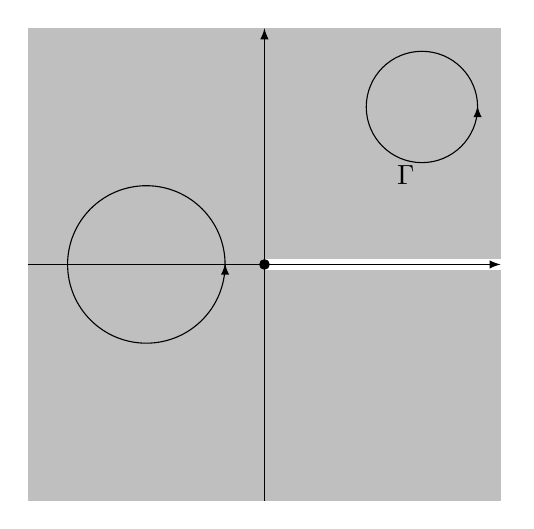
\begin{tikzpicture}
		\tikzset{> = latex}
		\filldraw [fill = lightgray,line width = 0pt,lightgray] (-3,-3) rectangle (3,3);
		\draw [line width = 3.8pt,white] (0,0) -- (3,0);
		\draw [->] (-3,0) -- (3,0);
		\draw [->] (0,-3) -- (0,3);
		\filldraw (0,0) circle (0.06);
		\draw (-1.5,0) circle (1);
		\draw (2,2) circle (0.707);
		\draw[->] (-0.5,0) --++ (0,0.01);
		\draw[->] (2.707,2) --++ (0,0.01);
		\node[label = south:{\(\Gamma \)}] at (1.8,1.5){};
	\end{tikzpicture}
\end{center}
如图,选择正实轴作为这条曲线,则先限定了 \(z\) 只能在灰色区域部分取(事实上完全可以在白色曲线上取),这其实是复平面挖掉了一条直线。这样由于不能绕支点一圈,因此就没有多值性。当然为了确定上面的点的具体的函数值,我还应该给出此时宗量的辐角范围或者灰色区域上任意一个点的值(支点不算)。而这条白色曲线作为分割辐角取值的作用(必然是分出 \(2\pi \) 长度的区间)称为\textbf{割线}。
\begin{itemize}
	\item 以上图作为例子,我规定宗量的辐角范围为 \([2\pi ,4\pi )\),这意味着若 \(z\) 在割线上,则我认为它的辐角是 \(2\pi \),\(z\) 在割线南端无穷小处,其辐角认为是 \(4\pi \),此时的辐角必然是不连续的,要考虑连续的辐角必须直面多值性。
\end{itemize}
接下来是另一些例子,由于支点可以不止有一个,考虑函数 \(f:z\mapsto \sqrt{(z-a)(z-b)}\),则此时 \(a,b\)  都是支点:

\begin{center}
	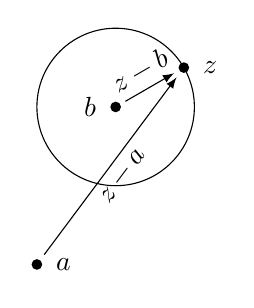
\begin{tikzpicture}
		\tikzset{> = latex}
		\draw (2,5) circle (1);
		\node[label = east:{\(a\)}] (A) at (1,3){};
		\node[label = west:{\(b\)}] (B) at (2,5){};
		\node[label = east:{\(z\)}] (Z) at (2.866,5.5){};
		\filldraw (A) circle (0.06);
		\filldraw (B) circle (0.06);
		\filldraw (Z) circle (0.06);
		\draw[->] (A) -- node[below,sloped]{\(z-a\)}(Z);
		\draw[->] (B) -- node[above,sloped]{\(z-b\)}(Z);
	\end{tikzpicture}
\end{center}

此时 \(z\) 绕圆周转一圈,势必会引起 \(\operatorname{Arg}_b(z)\) 改变 \(2\pi \),而 \(\sqrt{(z-a)(z-b)}\) 的辐角将会改变 \(\pi \)。因此 \(z-b\) 会引起多值性,此时 \(z-a,z-b\) 都是宗量,\(a,b\) 都是支点。

此时的割线依然要把握让 \(z\) 既不能绕 \(a\) 一圈也不能绕 \(b\) 一圈的职责:

\begin{center}
	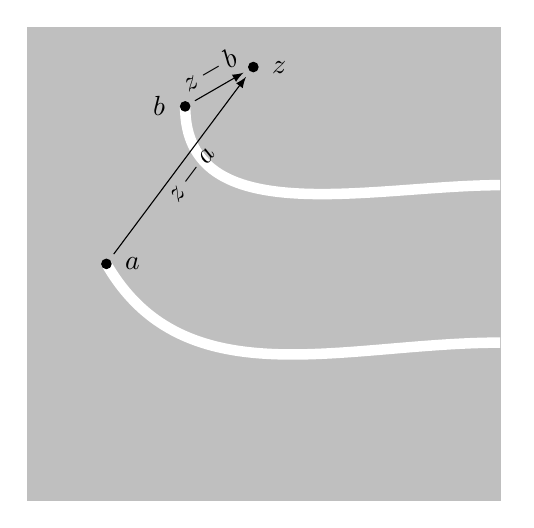
\begin{tikzpicture}
		\tikzset{> = latex}
		\filldraw[fill = lightgray,lightgray,line width = 0pt] (0,0) rectangle (6,6);
		\draw [line width = 3.8pt,white] (1,3) to [out=-60,in=180](6,2);
		\draw [line width = 3.8pt,white] (2,5) to [out=-90,in=180](6,4);
		\node[label = east:{\(a\)}] (A) at (1,3){};
		\node[label = west:{\(b\)}] (B) at (2,5){};
		\node[label = east:{\(z\)}] (Z) at (2.866,5.5){};
		\filldraw (A) circle (0.06);
		\filldraw (B) circle (0.06);
		\filldraw (Z) circle (0.06);
		\draw[->] (A) -- node[below,sloped]{\(z-a\)}(Z);
		\draw[->] (B) -- node[above,sloped]{\(z-b\)}(Z);
	\end{tikzpicture}
\end{center}
如图是一种割线的画法,但事实上我们可能更倾向于:
\begin{center}
	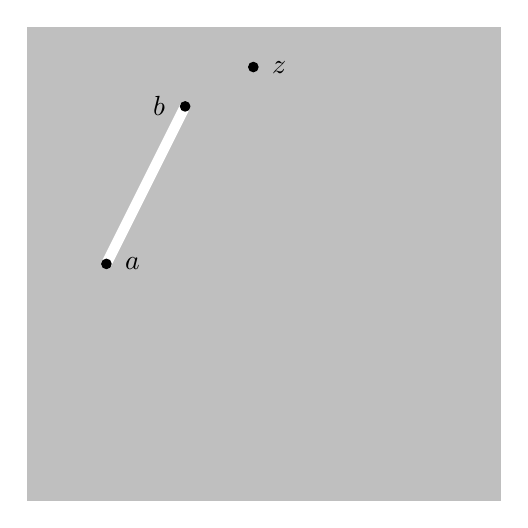
\begin{tikzpicture}
		\tikzset{> = latex}
		\filldraw[fill = lightgray,lightgray,line width = 0pt] (0,0) rectangle (6,6);
		\draw [line width = 3.8pt,white] (1,3) to (2,5);
		\node[label = east:{\(a\)}] (A) at (1,3){};
		\node[label = west:{\(b\)}] (B) at (2,5){};
		\node[label = east:{\(z\)}] (Z) at (2.866,5.5){};
		\filldraw (A) circle (0.06);
		\filldraw (B) circle (0.06);
		\filldraw (Z) circle (0.06);
	\end{tikzpicture}
	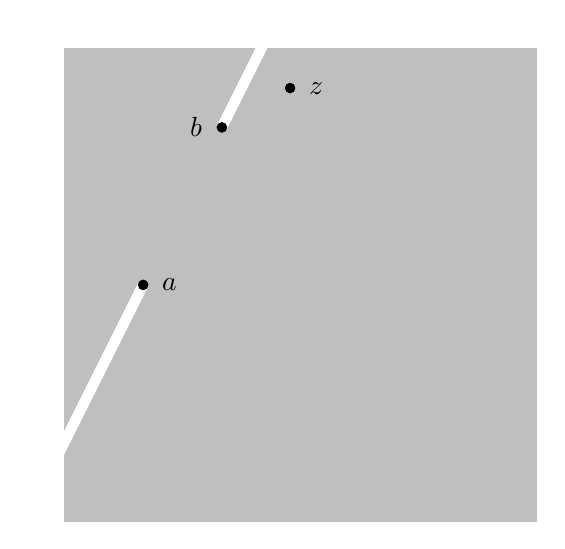
\begin{tikzpicture}
		\tikzset{> = latex}
		\filldraw[fill = lightgray,lightgray,line width = 0pt] (0,0) rectangle (6,6);
		\draw [line width = 3.8pt,white] (-0.4,0.2) to (1,3);
		\draw [line width = 3.8pt,white] (2,5) to (2.6,6.2);
		\node[label = east:{\(a\)}] (A) at (1,3){};
		\node[label = west:{\(b\)}] (B) at (2,5){};
		\node[label = east:{\(z\)}] (Z) at (2.866,5.5){};
		\filldraw (A) circle (0.06);
		\filldraw (B) circle (0.06);
		\filldraw (Z) circle (0.06);
	\end{tikzpicture}
\end{center}
这两种,具体情况以实际而定,要知道割线是会影响\textbf{收敛域}的。

此时我们在众多辐角各式各样的复平面中抽出了一个复平面出来,此被称为单值分支,如果函数是解析的,那就是单值解析分支。因此多值性可以认为是 \(z\) 从一个单值分支来到另一个单值分支引起的。不妨考虑将这些单值分支画出来连在一起:

\begin{center}
	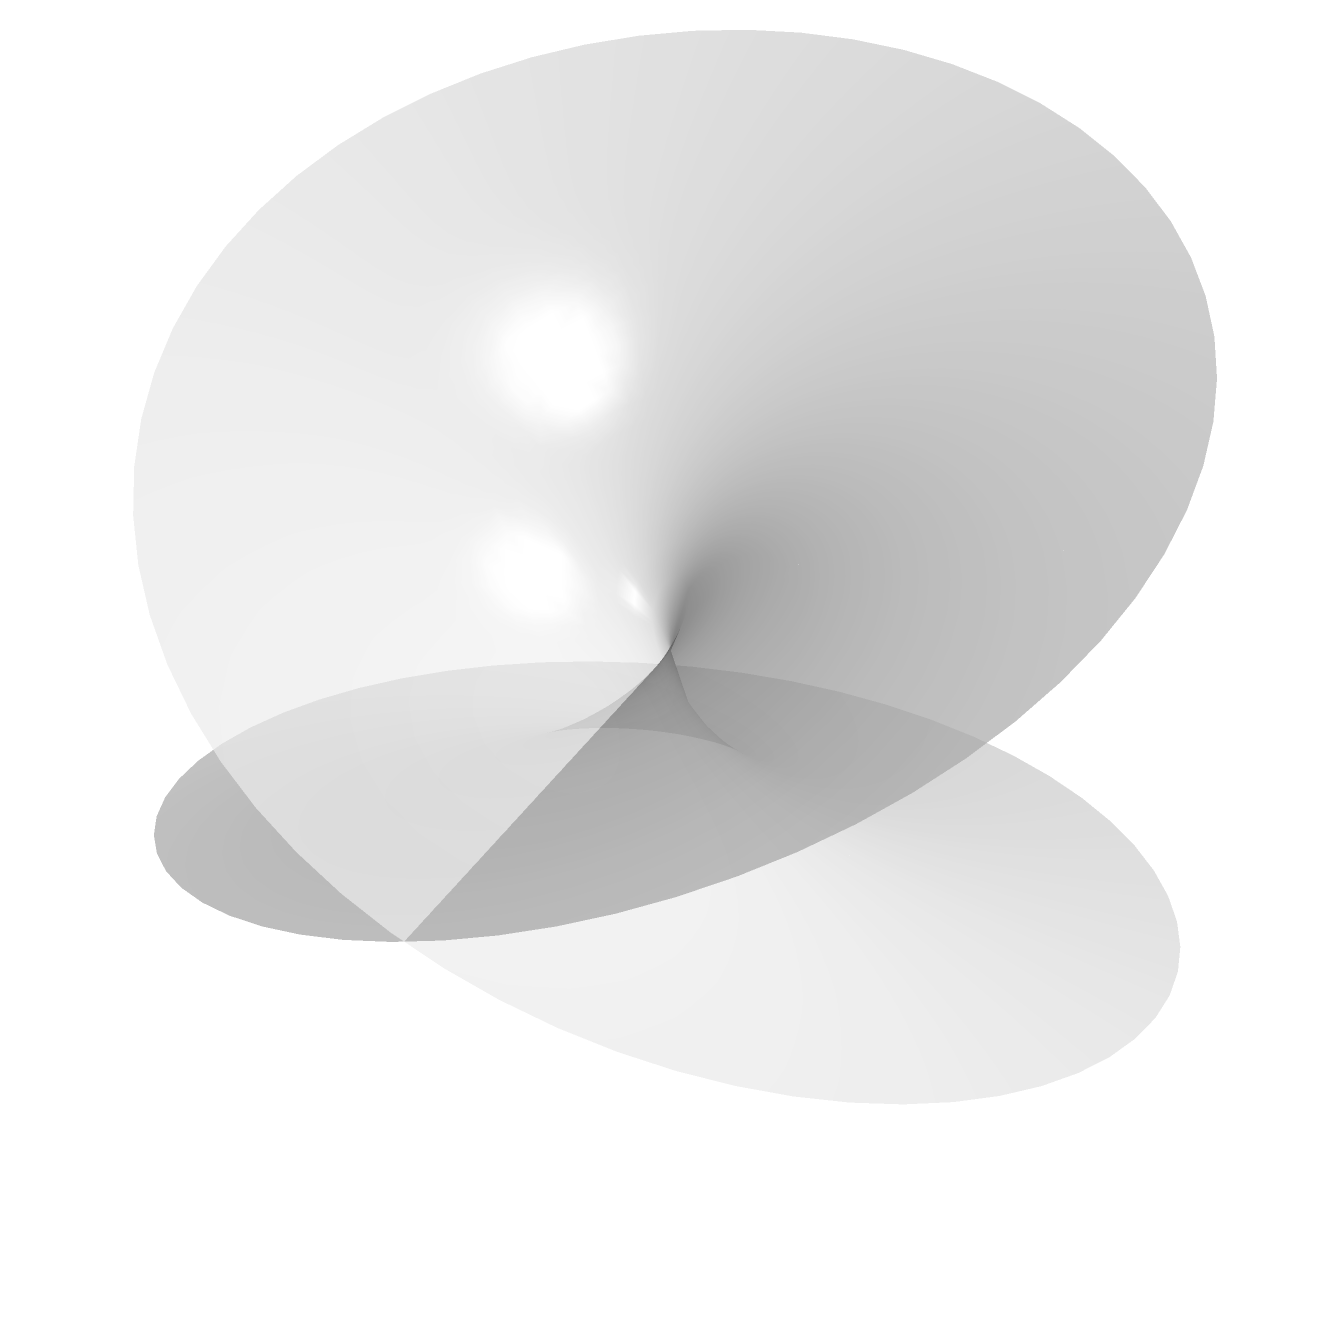
\includegraphics[width = 6cm]{Sqrt[z]@Rm.png}
\end{center}

这是 \(\sqrt{z}\) 的 \textbf{Riemann 面},\sout{意会即可}。下图是 \(\sqrt{(z-a)(z-b)}\) 的Riemann面\footnote{这里绘制Riemann面的程序来自\hyperref[https://resources.wolframcloud.com/FunctionRepository/resources/RiemannSurfacePlot3D]{https://resources.wolframcloud.com/FunctionRepository/resources/RiemannSurfacePlot3D}.}:
\begin{center}
	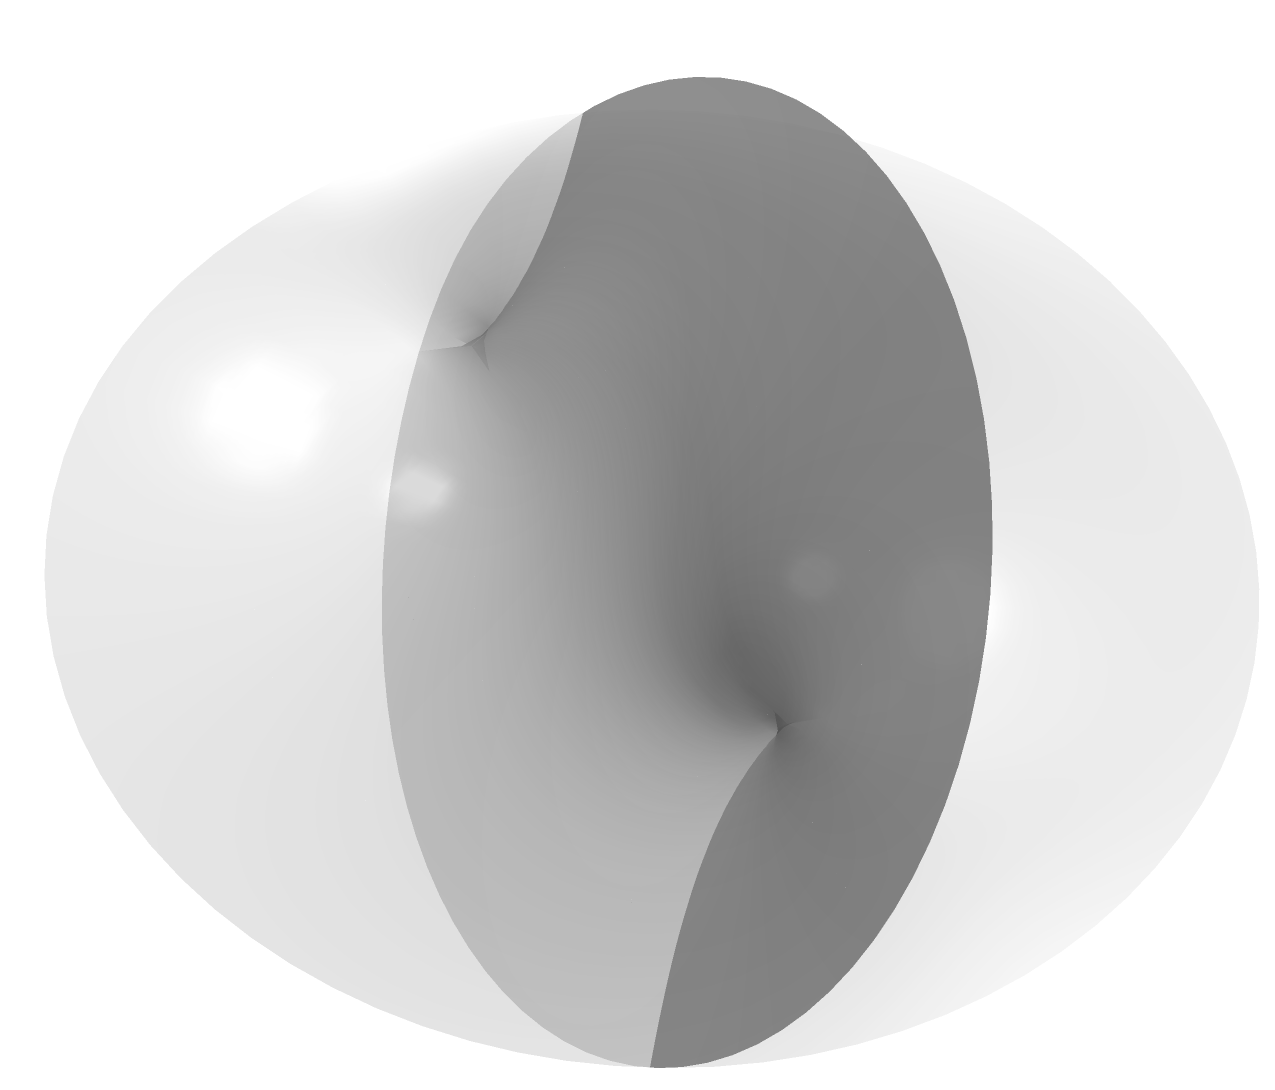
\includegraphics[width = 6cm]{Sqrt[(z-a)(z-b)]@Rm.png}
\end{center}

这是一种可视化多值函数的方法。注意到绕某个支点运动多次之后可以回到原来的分支,此时这些支点称为\textbf{代数支点}。

由此,我们根据在其中一个确定单值分支上面的 \(z\),再确立一条 \(z\) 的移动路线,我们就能够确立目的地所在的单值分支,进而确定函数值。接下来看些多值函数。

\begin{enumerate}
	\item 非整数幂函数 \(z^n,\,n\notin\symbb{Z} \),常见的多值函数,其单值分支在任意不包含割线和支点的区域内解析。因为一旦区域包含了支点,那必然直面多值性,而包含割线会导致不连续。
	      \[
		      \left( z^n \right) ' = nz^{n-1}
		      .\]
	      因此我们将之前幂级数那里的解析性表格改为:
	      \begin{center}
		      \begin{tblr}{
			      row{odd} = {bg=gray9},
			      colspec ={llllll},
			      row{1} = {bg = gray2, fg=white, font = \sffamily},
			      hline{1,Z} = {1pt},
					      vline{2} = {odd}{0.4pt,gray9},
					      vline{2} = {1}{0.4pt,black},
					      width = 0.9\textwidth,
					      colspec = {XX}
				      }
			      \textsf{\textit{n}} 是什么形状的 & \(\textsf{\textit{z}}^{\textsf{\textit{n}}}\) 的解析性                                      \\
			      \(n\in\symbb{N} \)               & \(z^n\) 在 \(\symbb{C} \) 上解析                                                            \\
			      \(n\in\symbb{N} ^-\)             & \(z^n\) 在 \(\symbb{C}\cup\left\{\infty  \right\} \setminus\left\{ 0 \right\}   \) 上解析。 \\
			      其他情况                         & \(z^n\) 在 \(\symbb{C} \setminus\left\{ 0 \right\} \) 且不包括割线的区域上解析。            \\
		      \end{tblr}
	      \end{center}
	\item 对数函数 \(\log z\),这里的底数是 \(\symrm{e} \coloneqq \lim_{n\to \infty}\left( 1+\frac{1}{n} \right) ^n\)。对数函数的定义是:满足 \(\symrm{e} ^ w = z\) 的所有值都称为 \(w = \log z\) 的值。考虑 \(z = r\symrm{e} ^{\symrm{i} \theta}\),则 \(\symrm{e}^{\log r+\symrm{i} \theta+2k \pi \symrm{i} } = r\symrm{e} ^{\symrm{i} \theta},\,k\in\symbb{Z} \),故:
	      \[
		      \symrm{e}^{\log r+\symrm{i} \theta+2k \pi \symrm{i} } \in \log z,\,k\in\symbb{Z}
		      .\]
	      同时也易得所有满足 \(\symrm{e} ^ w = z\) 都可以写成 \(\symrm{e}^{\log r+\symrm{i} \theta+2k \pi \symrm{i} }\) 的形式。因此对数函数可以认为是:
	      \[
		      \log z\coloneqq \log \left\vert z \right\vert +\symrm{i} \operatorname{Arg}_0(z)
		      .\]
	      注意到 \(\operatorname{Arg}_0(z)\) 可以以 \(2\pi \) 为距离在 \(\symbb{R} \) 上游走,因此 \(\log z\) 的多值性体现在其虚部。
	      \begin{center}
		      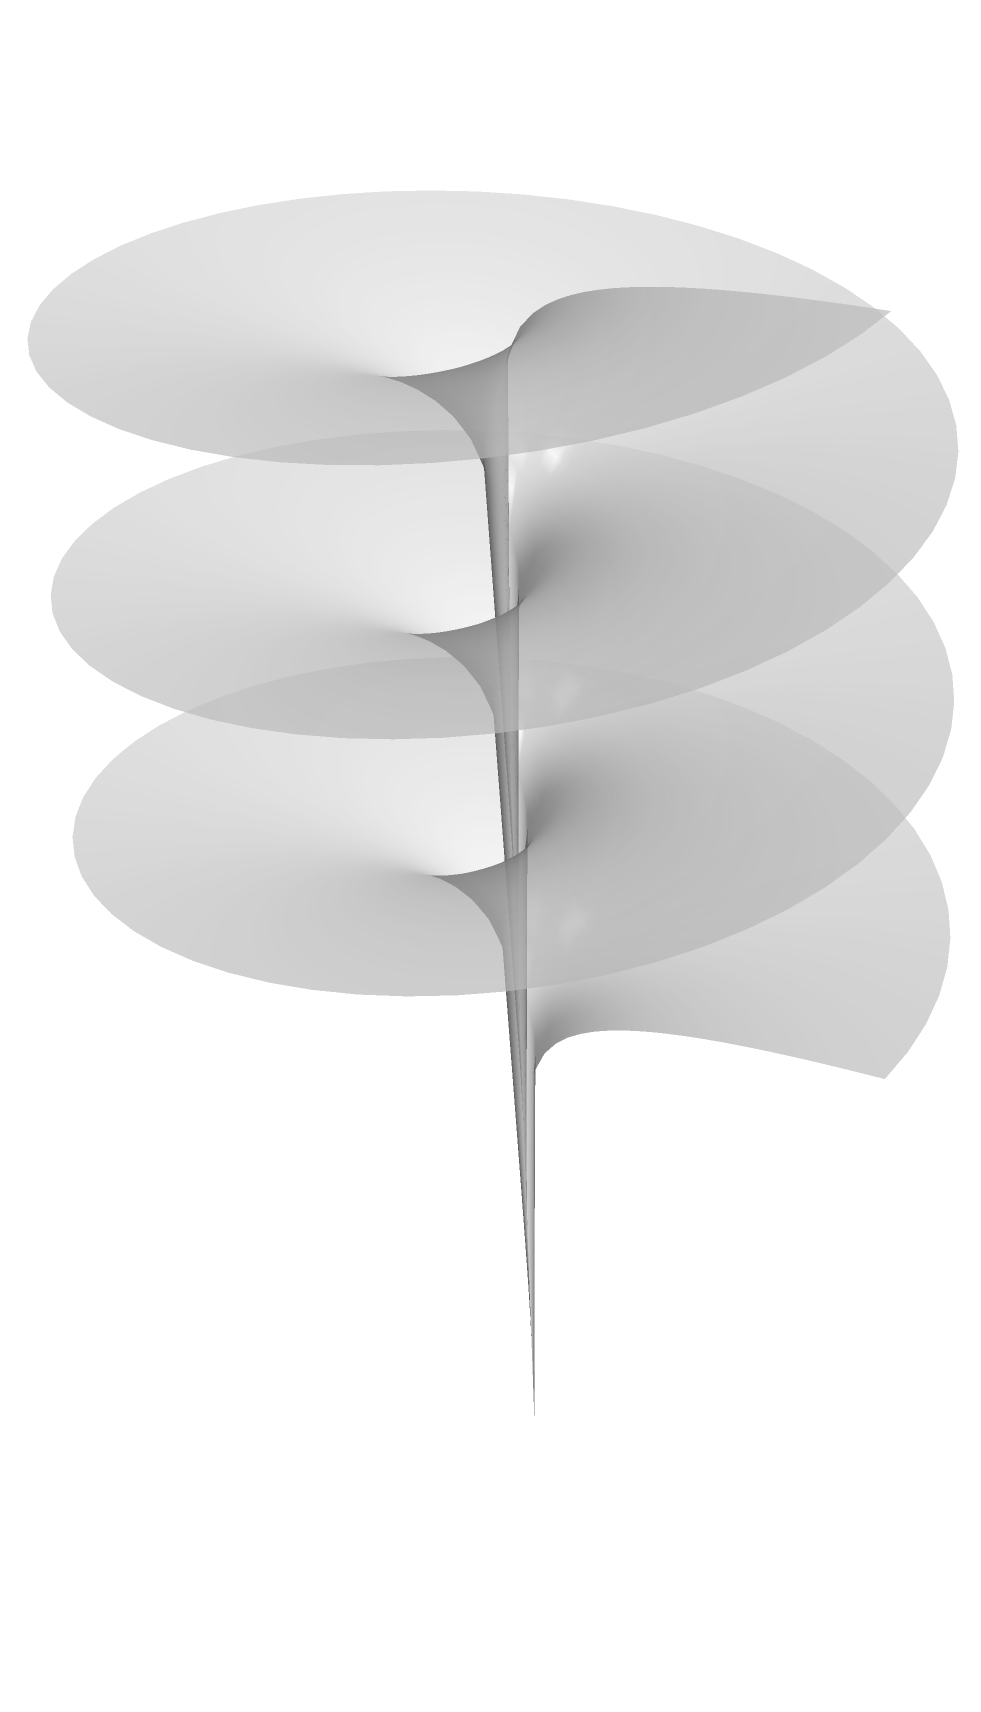
\includegraphics[width = 6cm]{Log[z]@Rm.png}
	      \end{center}
	      上图是 \(\log z\) 的Riemann图。此时无论绕支点旋转多少次都回不到原来的分支,这样的支点称为\textbf{对数支点}。

	      上面的非整数幂函数 \(z^n\) 可以表示为 \(\symrm{e} ^{n \log z}\)。
	\item 反三角/双曲函数:
	      \[
		      \begin{cases}
			      \arcsin z\coloneqq -\symrm{i} \log \left(\symrm{i} z+\sqrt{1-z^2 } \right) =-\symrm{i} \operatorname{arcsinh}\left( \symrm{i}z\right), \\
			      \arccos z \coloneqq  -\symrm{i} \log \left( z+\sqrt{z^2-1} \right)=-\symrm{i} \operatorname{arccosh} z,                                          \\
			      \arctan z\coloneqq -\frac{\symrm{i} }{2}\log \left( \frac{1+\symrm{i} z}{1-\symrm{i} z} \right) =\symrm{i} \operatorname{arctanh}(\symrm{i} z).
		      \end{cases}
	      \]
\end{enumerate}
至于这些函数的求导,按照实变量的函数求导即可。

\subsection{其他废话}
有多值函数那边看出,这些初等多值函数都是某些函数的反函数,而这些函数或多或少有\textbf{多对一}的情况。因此若考虑以下性质的函数:
\[
	\forall z_1,z_2\in I,\,f(z_1)\neq f(z_2)
	.\]
则称 \(f\) 在 \(I\) 上是\textbf{单叶}的。如果解析函数 \(f\) 满足:
\[
	f:I_1\to I_2\,\mbox{\it 且}\, f\,\mbox{\it 是单叶的}
	.\]
则存在单叶解析的反函数 \(f^{-1} :I_2\to I_1\),此时的 \(f\) 称为\textbf{共形映射}。更进一步地,如果 \(f\) 在 \(I\) 上是单叶解析函数,则 \(f'(z)\) 在 \(I\) 上处处不为零。
\section{幂级数}
TODO。
\end{document}
